%% International Journal of Computational Intelligence Systems ---
%%%%%%%%%%%%%%%%%%%%%%%%%%%%%%%%%%%%%%%%%%%%%%%%%%%%%%%%%%%%%%%%%%%%%%%%%%%
\documentclass[11pt,twoside]{article}
\usepackage{ijcis}
%--------------------- ADDITIONAL PACKAGES HERE ---------------------------
\usepackage{amsmath}
\usepackage{amssymb}
\usepackage{color}

\hyphenation{pro-per-ties}
\hyphenation{ge-ne-ral-ly}
\hyphenation{pre-fe-ren-ces}
\hyphenation{u-sing}
\hyphenation{pu-nish-ment}
\newcommand{\Pow}{\mathcal{P}}
\newcommand{\N}{\operatorname{N}}
\newcommand{\bool}{\operatorname*{\mathcal{B}}}
\newcommand{\Pos}{\operatorname{Pos}}
\newcommand{\Nec}{\operatorname{Nec}}
\newcommand{\Open}{\operatorname{Open}}
\newcommand{\Rp}{\operatorname{Rp}}
\newcommand{\Rn}{\operatorname{Rn}}
\newcommand{\FB}{\operatorname{FB}}
\newcommand{\UC}{\operatorname{UC}}
\newcommand{\T}{\mathcal{T}}
\newcommand{\C}{\mathcal{C}}
\newcommand{\Nat}{\mathbb{N}}
\newcommand{\Q}{\mathbb{Q}}
\newcommand{\R}{\mathbb{R}}
\newcommand{\Z}{\mathbb{Z}}
\newcommand{\Head}{\mathcal{H}}
\newcommand{\Body}{\mathcal{B}}
\newcommand{\Dom}{\mathcal{D}}
\newcommand{\INS}{\mbox{\textbf{insert}}}
\newcommand{\DEL}{\mbox{\textbf{delete}}}
\newcommand{\MOD}{\mbox{\textbf{modify}}}
\newcommand{\Overlap}{\mbox{\textbf{Overlap}}}
%--------------------------------------------------------------------------
%
\def\labart{yourLabel}      % put a label from your choice here
%\Vol{1}                    % number of the Volume
%\Issue{1}                  % number of the issue
%\Month{January}            % month
%\Year{2008}                % year
%\received{...}
%\revised{...}
%
%---------------------------------------------------------------------------
\thispagestyle{empty}
%%------------------------- YOUR HEADINGS HERE -----------------------------
% Author's initials of first names+last names
\shortauthors{J. Pons}
% Short title
\shorttitle{A possibilistic general valid-time model}
%---------------------------------------------------------------------------
%
%---------------------- YOUR TITLE ----------------------------------------
\title{A Possibilistic Valid-time Model 
 \\ \vspace*{0.04truein}
%Using \LaTeX\footnote{For the title, try not to use more than 3 lines.
%Typeset the title in 12 pt Times Roman, uppercase and boldface.}
}
%-------------------------- AUTHOR'S NAMES ----------------------------------
\author{%
Jose Enrique Pons\,\up{1}\,\,,Olga Pons\,\up{1}\,\,
%\author{
Christophe Billiet\,\up{2}\,,Guy de Tr\'{e}\,\up{2}\,
}
%----------------------------- ADDRESSES ----------------------------------
\addresses{%
%\address{
\up{1}
Department of Computer Science and Artificial Intelligence, University of Granada\\
C/ Periodista Daniel Saucedo Aranda, S/N,E-18071\\
Granada, Spain%
\footnote{
Jos\'e Enrique Pons Fr\'ias, Universidad de Granada, C/ Periodista Daniel Saucedo Aranda S/N, E-18071, Granada, Spain.
%State completely without abbreviations, the affiliation
%and mailing address, including country. Typeset in 10~pt Times Italic.
}
\\ \vspace*{0.04truein}
E-mail: jpons,opc@decsai.ugr.es
%}\address{%
\\ \vspace*{0.05truein}
\up{2}
Department of Telecommunications and Information Processing, Ghent University \\
Sint-Pietersnieuwstraat 41 B-9000, Ghent, Belgium.
\\ \vspace*{0.04truein}
E-mail: Christophe.Billiet,Guy.De.Tre@ugent.be
}
%---------------------------------------------------------------------------
\pagestyle{myheadings}
\begin{document}
\label{\labart-FirstPage}

\maketitle
%-------------------------- ABSTRACT ---------------------------------------
\abstracts{
%%%%%%%%%%%%%%%%%%%%%%%%
%
% ABSTRACT
%
%%%%%%%%%%%%%%%%%%%%%%%%
In reality, some objects or concepts have properties with a time-variant or time-related nature. Modelling these kinds of objects or concepts in a (relational) database schema is possible, but time-variant and time-related attributes have an impact on the consistency of the entire database. Therefore, temporal database models have been proposed to deal with this. Time itself can be at the source of imprecision, vagueness and uncertainty, since existing time measuring devices are inherently imperfect. Accordingly, human beings manage time using temporal indications and temporal notions, which may contain imprecision, vagueness and uncertainty. However, the imperfection in human-used temporal indications is supported by human interpretation, whereas information systems need support for this. Several proposals for dealing with such imperfections when modelling temporal aspects exist. Some of these proposals transform the temporal expression into a compact representation. Other proposals consider the temporal indications in the used temporal expressions to be the source of imperfection. 
In this work we present a novel model to deal with imperfections in valid-time databases. Next to that, the data manipulation language, \emph{DML} is defined and implemented.%
%The abstract should summarize the context, content and conclusions of the
%paper in less than 80 words. It should not contain any references or
%displayed equations. Typeset the abstract in 9~pt Times Roman with
%baselineskip of 11 pt, making an indentation of 2.5 picas on the left
%and right margins.
}
\par\bigskip\par
%-------------------------- KEYWORDS ---------------------------------------
\keywords{possibilistic, fuzzy temporal, database, valid time}

\vspace*{10pt}\textlineskip
%-------------------------- BEGIN BODY OF TEXT -----------------------------
\begin{multicols}{2}

\section{\label{sec:intro}Introduction}
%%%%%%%%%%%%%%%%%%%%%%%%%%%%%%%%%%%%%%%%%%%%%%%%%%%%%%%%%%%%%%%%%%%%%%
%
% Introduction
%
%%%%%%%%%%%%%%%%%%%%%%%%%%%%%%%%%%%%%%%%%%%%%%%%%%%%%%%%%%%%%%%%%%%%%%

The concept of time is very complex to handle and interpret~\cite{Klein1994,Shackle1961}, though it is very natural and omnipresent in real world data. As information systems attempt the modelling of natural objects, concepts or processes, they often require modelling temporal aspects or concepts. Thus, several proposals have arisen to obtain theoretical models that allow the modelling or representation of time~\cite{Bolour1982,VanderCruyssen1997}.

A very specific type of information systems are database systems. A database contains data representing real objects or concepts. In real world, some aspects or properties of objects are time-variant or time-related. e.g., the moment of a bank transaction and the status of an employee in a company, are time-related and time-variant notions, respectively.
A temporal database schema is a database schema that models objects with time-related or time-variant properties. However, the modelling of temporal aspects has a direct impact on the consistency of the temporal database, because the temporal nature of these aspects imposes extra integrity constraints and suitable ways of interactive with the human user. 

For example, let us consider a hospital database containing data about the state of the patients in a given hospital. Two dates are stored: the date when the patient arrives to and leaves from the hospital. It is clear that a patient cannot leave the hospital if he or she has not arrived. Without further cautions, a hospital employee could insert a patient who is already in the hospital. A temporal database model will typically constrain record insertion and prevent similar modelling inconsistencies.

A lot of research concerns temporal database models and their approaches to the modelling of time. The first efforts were towards the representation of historical information related to objects represented by records in a database~\cite{Clifford1985}. Some proposals tried to extend the Entity Relationship Model~\cite{Klopprogge1983}, without impact on any database standards like SQL~\cite{Sarda1990}.

Notably, in 1994, ``A Consensus Glossary of Temporal Database Concepts'' was published~\cite{Dyreson1994}. For this publication, 44 temporal database researchers, among them, some of the main researchers in this field, cooperated to reach a consensus on the nature and definitions of some of the main temporal database concepts and terminology. This glossary was updated in 1998~\cite{Dyreson1998}.


% %From time in general to time in information systems
% In real world, some aspects or properties of objects, concepts or processes are time-variant or time-related. For example, the moment of a bank transaction is traditionally a point in time and thus a time-related notion, the function of an employee in a company can change through recorded history and is thus time-variant.  As information systems often attempt the modelling of natural objects, concepts or processes, they often require modelling temporal aspects or concepts. Thus, several proposals have been concerned with obtaining theoretical models that allow the modelling or representation of time~\cite{Bolour1982},~\cite{VanderCruyssen1997}.

% %From time in information systems to time in temporal databases
% Time is a complex concept, which makes modelling time in database systems complex too. A \emph{temporal database} is a database that deals with certain time-related aspects in its schema: a \emph{temporal database schema}~\cite{Dyreson1994} is a database schema that models entities (and interactions or relationships between entities) with time-related or time-variant properties. However, the modelling of temporal properties or aspects has a direct impact on the consistency of the resulting temporal database, because the temporal nature of these aspects or properties imposes extra integrity constraints. An example. Consider a relation in a relational library database, representing the physical absence (or presence) of books in the library. Every physical book is represented by a unique identifier. Every record in the relation contains such an identifier, a date on which the corresponding book was loaned and a date on which it was subsequently returned (if it was returned). As such, every record represents a period of time during which the physical book corresponding with the identifier is loand to a library customer. Without further precautions, a library employee could add several records with the same book identifier, different `loaned'-dates and no `returned'-dates. This group of records would represent the same physical book being loaned several times on different dates and never returned, which is of course impossible. A temporal database model will typically constrain record insertion and prevent similar modelling inconsistencies.

An interesting issue in temporal modelling concerns relationships between temporal notions. In this sense, Allen~\cite{Allen1983} studied temporal relationships between time intervals (and as a special case time points). Among others, the querying of temporal databases has greatly profited from these temporal relationships, because they allowed more powerful user-specified temporal query demands, by allowing to express more complex relationships between the temporal notions in the temporal expressions in the query. For example, a query like `who were the department heads when Thomas worked for the institution' can be evaluated using operators similar to Allen's ones.

Humans handle temporal information using certain temporal notions like time intervals or time points~\cite{Dyreson1994}, and they often have to deal with imperfections like imprecision, vagueness, uncertainty or inconsistencies possibly contained in the descriptions of these temporal notions. These possible imperfections in descriptions of temporal notions determine an important issue in temporal modelling. Consider as an example the description of the temporal notion in a sentence like `The Belfry of Bruges was finished between 01/01/1201 A.D. and 31/12/1300 A.D.'. These sentence contains imperfection because of the uncertainty in the used time-related expression. It is known that the building was finished on a single day, but this day is not precisely known.

To allow information systems to cope with these and similar data imperfections, many approaches adopt fuzzy sets~\cite{Zadeh1965} for the representation and management of temporal information~\cite{Mitra1994,Nagypal2003,Billiet2011,Dubois2003}. The temporal relationships studied by Allen were fuzzified by several authors~\cite{Ohlbach2004,Nagypal2003,Schockaert2008}.   Garrido et al. ~\cite{Garrido2009} presented a compact representation for the time and defined different relationships among time intervals by using a combination of regular fuzzy comparisons. Also ~\cite{Garrido2009,Pons2011} studied uncertainty in temporal expressions concerning time intervals. Other approaches, like~\cite{Qiang2009}, use rough sets~\cite{Pawlak1995} to represent time intervals.

%Now introducing imperfections in representations of time...
% Humans handle temporal information using certain temporal notions like specific time intervals or instants~\cite{Dyreson1994} and they often have to deal with imperfections like imprecisions, vaguenesses, uncertainties or inconsistencies possibly contained in (the descriptions of) these temporal notions. Among many others, these possible imperfections in (descriptions of) temporal notions determine an important issue in temporal modelling. As an example, consider the temporal notion described in a sentence like `The Belfry of Bruges was finished on a day somewhere between 01/01/1201 A.D. and 31/12/1300 A.D.'. The description of the temporal notion reads `a day somewhere between 01/01/1201 A.D. and 31/12/1300 A.D.'. This temporal notion thus contains imperfection in the form of the uncertainty about the exact day the last stone of the building was laid: it is known that the building was finished on a single day, but it is not known which day this was. To allow information systems to cope with these and similar temporal data imperfections, many approaches adopt fuzzy sets~\cite{Zadeh1965} and/or fuzzy logic to model temporal information~\cite{Mitra1994},~\cite{Nagypal2003},~\cite{Billiet2011},~\cite{Dubois2003}. 

In addition to temporal modelling, some attention has been paid to temporal reasoning~\cite{Allen1983}. Although temporal reasoning is not discussed in this paper, it should be noted that, among others, Dubois and Prade et al.~\cite{Dubois2003,DuBois1989} have dealt with fuzziness and uncertainty in temporal reasoning.

The present work defines and implement a model for properly represent and manage uncertainty in valid-time specification in a relational database. Our work is focused on both the proposal of an appropriate formal framework to suitably manage time in databases and the implementation of an DML that allows to the user the transparent use of this proposal. None of the previous research offer a database model to accomplish this task.

This way together with the theoretical model, we also present and explain the main operations of the manipulation language for a temporal database which stores the valid-time periods of the objects affected by imprecision. The rest of the work is organized as follows. Section \ref{sec:prelim} presents some background concepts about both possibility theory and temporal databases. In section \ref{sec:time-rep} the representation of the valid-time intervals in the database is explained. Section \ref{sec:temporal-model} explains the main concepts of the temporal Data Manipulation Language (DML) and its implementation. Finally, Section \ref{sec:conclusions} presents the conclusions and some guidelines for future research work.


% 
% 
% %From information systems in general to database systems in particular:
% Generally, \emph{information systems} model the structure and behavior of real objects, concepts or processes. A specific type of information systems are \emph{database systems}, which are computer systems designed to manage \emph{databases}. A database is basically a collection of (persistent) data. These (typically atomic) data represent real objects or concepts. In the context of database design, such objects or concepts are typically called \emph{entities} and a collection of similar entities is typically modelled by an \emph{entitytype}, which is basically a combination of a name and a list of \emph{attributes}, which describe properties of the entities. Typically, in an early stage of the database development process, the structures of and interactions or relationships between used entities are modelled in a \emph{design schema}, following some design model. A database thus contains (typically atomic) data. Each (atomic) part of these data is a result value of a measurement of a property of an entity or a description of a property of an entity and will correspond to the attribute of the entity's entitytype, which describes the property.
% 
% %From database models in general to the relational model in particular:
% The structure and behavior of a database, along with some integrity and security restrictions, is dictated by a \emph{database model}. A database model is basically a collection of instructions and regulations, used to (logically) describe the structure and behavior of a database, along with some integrity and security restrictions. Applying a database model to a concrete design schema results in a \emph{database schema}, which models the logical structure and behavior of a database. Several different database models exist, but the most popular is the \emph{relational database model}~\cite{Codd:1970:RMD:362384.362685}. Following the relational database model, entitytypes are modelled as \emph{relations}, which comprise a name and a list of attributes, modelling the entitytype's attributes.
% 
% %From time in general to time in information systems
% In reality, some aspects or properties of objects, concepts or processes are time-variant or time-related. For example, the moment of a bank transaction is traditionally a moment in time and thus a time-related notion, the function of an employee in a company can change through recorded history and is thus time-variant. The concept of time itself is very complex to handle and interpret~\cite{Klein1994},~\cite{Shackle1961}, though it is very natural and omnipresent. As information systems often attempt the modelling of natural objects, concepts or processes, they often require modelling temporal aspects or concepts. Thus, several proposals have been concerned with obtaining theoretical models that allow the modelling or representation of time~\cite{Bolour1982},~\cite{VanderCruyssen1997}.
% 
% %From time in information systems to time in temporal databases
% Time is a complex concept, which makes modelling time in database systems complex too. A \emph{temporal database} is a database that deals with certain time-related aspects in its schema: a \emph{temporal database schema}~\cite{Dyreson1994} is a database schema that models entities (and interactions or relationships between entities) with time-related or time-variant properties. However, the modelling of temporal properties or aspects has a direct impact on the consistency of the resulting temporal database, because the temporal nature of these aspects or properties imposes extra integrity constraints. An example. Consider a relation in a relational library database, representing the physical absence (or presence) of books in the library. Every physical book is represented by a unique identifier. Every record in the relation contains such an identifier, a date on which the corresponding book was loaned and a date on which it was subsequently returned (if it was returned). As such, every record represents a period of time during which the physical book corresponding with the identifier is loand to a library customer. Without further precautions, a library employee could add several records with the same book identifier, different `loaned'-dates and no `returned'-dates. This group of records would represent the same physical book being loaned several times on different dates and never returned, which is of course impossible. A temporal database model will typically constrain record insertion and prevent similar modelling inconsistencies.
% 
% %Research about temporal databases
% A lot of research concerns temporal database models and their approaches to the modelling of time. Some of the first proposals concerned the representation of historical information related to entities~\cite{Clifford1985}. Some proposals tried to extend the Entity Relationship Model~\cite{Klopprogge1983}, without impact on any database standards like SQL~\cite{Sarda1990}. Notably, in 1994, `A Consensus Glossary of Temporal Database Concepts' was published~\cite{Dyreson1994}. For this publication, 44 temporal database researchers, among which some of the main researchers in this field, cooperated to reach a consensus on the nature and definitions of some of the main temporal database concepts and their terminology. This glossary was subsequently updated in 1998~\cite{Dyreson1998}. In the presented work, the concepts and terminology from this glossary are used and followed.
% 
% %Research about temporal relationships
% An interesting issue in temporal modelling concerns the relationships between temporal notions. Notably, Allen~\cite{Allen1983} studied temporal relationships between time intervals~\cite{Dyreson1994} (and, as a special case, instants~\cite{Dyreson1994}). Among others, the querying of temporal databases has greatly profited from these temporal relationships, because they allow for richer and more complex user-specified temporal query demands, by allowing to express more complex relationships between the temporal notions in the temporal expressions in the query and the temporal indications in the database. For example, given a relation representing who was department head of an institution during which time intervals, a query like `Who were the department heads during the time intervals when Thomas worked for the institution?' can be evaluated using similar relationships. %TODO: CHECK THIS LAST SENTENCE
% 
% %Now introducing imperfections in representations of time...
% Humans handle temporal information using certain temporal notions like specific time intervals or instants~\cite{Dyreson1994} and they often have to deal with imperfections like imprecisions, vaguenesses, uncertainties or inconsistencies possibly contained in (the descriptions of) these temporal notions. Among many others, these possible imperfections in (descriptions of) temporal notions determine an important issue in temporal modelling. As an example, consider the temporal notion described in a sentence like `The Belfry of Bruges was finished on a day somewhere between 01/01/1201 A.D. and 31/12/1300 A.D.'. The description of the temporal notion reads `a day somewhere between 01/01/1201 A.D. and 31/12/1300 A.D.'. This temporal notion thus contains imperfection in the form of the uncertainty about the exact day the last stone of the building was laid: it is known that the building was finished on a single day, but it is not known which day this was. To allow information systems to cope with these and similar temporal data imperfections, many approaches adopt fuzzy sets~\cite{Zadeh1965} and/or fuzzy logic to model temporal information~\cite{Mitra1994},~\cite{Nagypal2003},~\cite{Billiet2011},~\cite{Dubois2003}. 
% 
% %Now introducing imperfections in temporal relationships
% The temporal relationships studied by Allen were fuzzified by several authors~\cite{Ohlbach2004},~\cite{Nagypal2003},~\cite{Schockaert2008}. Garrido et al. ~\cite{Garrido2009} present different temporal operators, defined by a combination of fuzzy comparisons. Also,~\cite{Garrido2009},~\cite{Pons2011} studied uncertainty in the context of time intervals. Other approaches, like~\cite{Qiang2009}, use rough sets~\cite{Pawlak1995} to represent time intervals.
% 
% %Imperfections in temporal reasoning
% Next to temporal modelling, some attention has gone to temporal reasoning~\cite{Allen1983}. Although the focus of this paper is temporal modelling, it should be noted that, among others, Dubois and Prade et al.~\cite{Dubois2003},~\cite{DuBois1989} have dealt with fuzziness and uncertainty in temporal reasoning.
% 
% %Overview of this work
% %Include: what is the paper about? (situation and explanation of the problem we will solve and situation of our solution (we use constraints...))
% %Include: how does the solution work? (short summary of how the solution will solve the problem/attend to the problem)
% %Include: What exactly will be presented
% %In all of these: stress every single innovative/novel point of the presented work!
% %TODO: build the overview when the paper is finished
% 
% The aim of this work is to present and explain the main operations of the manipulation language for a temporal database which stores the valid-time periods of the objects with uncertainty. The rest of the work is organized as follows. Section \ref{sec:prelim} presents some background concepts about both possibility theory and temporal databases. In section \ref{sec:time-rep} the representation of the valid-time intervals in the database is explained. Section \ref{sec:temporal-model} explains the main concepts and behaviour of the temporal model. The Data Manipulation Language (DML) is described and implemented. Finally in Section \ref{sec:conclusions} presents the conclusions and some possibilities for future research work.
% 



\section{\label{sec:prelim}Preliminaries}
%Introductory text:
In this section, some basic concepts are introduced, concerning possibility theory, possibilistic variables and fuzzy numbers and intervals. The framework of set evaluation by ill-known constraints\cite{Pon11} is explained. The section concludes with a brief introduction to temporal databases.

\subsection{\label{subsec:possibility-theory}Possibility Theory}
Possibility theory, like probability theory, deals with uncertainty about the outcome of an experiment. In probability theory, this uncertainty is caused by the \emph{variability} in the outcomes, while in possibility theory, the uncertainty is caused by \emph{incomplete knowledge} about the experiment. The quantification of confidence in a theory of uncertainty is achieved using a confidence measure\cite{Shafer:1976:AMathematical}. In probability theory this is a measure of chance, in possibility theory, possibility and necessity measures are used.

\begin{definition}
Consider a set of outcomes $\Omega$. Let $\wp(\Omega)$ denote the powerset of $\Omega$ and let $A$ and $B$ be elements of $\wp(\Omega)$. A \emph{confidence measure on $\Omega$} is defined by a function
	\begin{align}
	g : \wp(\Omega) & \rightarrow \left[0,1\right]
	\end{align}
that satisfies
	\begin{align}
	g(\emptyset) &= 0 \\
	g(\Omega) &= 1 	\label{NormalizationProperty} \\
	A \subseteq B &\Rightarrow g(A) \leq g(B) \label{MonotonicityProperty}
	\end{align}
\end{definition}

Both possibility measures and necessity measures are special cases of confidence measures.

\begin{definition}
Consider a confidence measure $\Pi$ on a set of outcomes $\Omega$. Let $J$ be a countable index set and let $\{ A_{j} | j \in J \wedge A_{j} \subseteq \Omega \}$ be a family of elements of $\wp(\Omega)$. $\Pi$ is now a \emph{possibility measure on $\Omega$} if it satisfies:
	\begin{align}
	\Pi\left(\bigcup_{j \in J} A_{j} \right) = \sup_{j \in J} \Pi(A_{j})
	\end{align}
\end{definition}

In this work, the interpretation is as follows. The possibility of an event expresses how plausible the occurrence of the event seems to an observer of the experiment, given the (partial) knowledge of the observer about the experiment.

Information on the possibility of distinct elements of the universe of discourse $\Omega$ can now be given by a \emph{possibility distribution} $\pi$ on $\Omega$, defined by:

\begin{definition}
Consider a possibility measure $\Pi$ on $\Omega$. A \emph{possibility distribution} $\pi$ on $\Omega$ underlying the possibility measure $\Pi$ is then a function defined by:
	\begin{align}
	\pi : \Omega \rightarrow \left[0, 1\right] : \pi(u) = \Pi(\{u\})
	\end{align}
\end{definition}

\begin{definition}
Consider a confidence measure $N$ on a set of outcomes $\Omega$. Let $J$ be a countable index set and let $\{ A_{j} | j \in J \wedge A_{j} \subseteq \Omega \}$ be a family of elements of $\wp(\Omega)$. $N$ is now a \emph{necessity measure} on $\Omega$ if it satisfies:
	\begin{align}
	N\left(\bigcap_{j \in J} A_{j} \right) = \inf_{j \in J} N(A_{j})
	\end{align}
\end{definition}

In this work, the interpretation is as follows. The necessity of an event expresses how necessary the occurrence of the event seems to an observer of the experiment, given the (partial) knowledge of the observer about the experiment.

Possibility and necessity measures are dual in the sense that:

\begin{align}
\forall A \subseteq \Omega : N(A) = 1 - \Pi(\bar{A})
\end{align}

Regarding interpretation, the above can be seen as: the degree to which an event is necessary is the degree to which every other possible event is not plausible.

\subsection{\label{subsec:possibilistic-variables}Possibilistic Variables}
A \emph{possibilistic variable} is defined as follows\cite{Pon11}.

\begin{definition}
A possibilistic variable $X$ over a universe $U$ is defined as a variable taking exactly one value in $U$, but for which this value is (partially) unknown. Its possibility distribution $\pi_X$ on $U$ gives the available knowledge about the value that $X$ takes: for each $u\in U$, $\pi_X(u)$ represents the possibility that $X$ takes the value $u$.
\end{definition}

The exact value a possibilistic variable takes, which is (partially) unknown, is called an \emph{ill-known value} in this work\cite{Dubois88b}.

When a possibilistic variable is defined on the powerset $\Pow(R)$ of some universe $R$, the unique value the variable takes will be a crisp set and its possibility distribution on the powerset $\Pow(R)$ will describe the possibility of each crisp subset of $R$ to be the value the variable takes. This exact value (a crisp set) the variable takes, is now called an \emph{ill-known set}\cite{Dubois88b}.

%It is important to understand the difference between the following two concepts:
%\begin{itemize}
%\item
%A \emph{possibilistic variable} $X$ is bounded to take only one value , but this value is not known due to incomplete knowledge. 
%\item
%An \emph{ill-known set}~\cite{Dubois88b}: a possibilistic variable defined over the universe $\Pow(U)$.
%\end{itemize}

%Note that while a possibilistic variable refers to one (partially) unknown value, an ill-known set is a crisp set but, for some reason, (partially) unknown.

A specific application of possibilistic variables is obtained when the universe under consideration is the set of boolean values $\mathbb{B}$ = $\{T,F\}$. Indeed, any boolean proposition $p$ takes just one value in $\mathbb{B}$. If the knowledge on which value this proposition $p$ will take is given by a possibility distribution $\pi_p$, the proposition can be seen as a possibilistic variable. As the interest lies with the case where the proposition holds, the possibility and necessity that $p$ = $T$ (the proposition holds) demand most attention. This possibility and necessity is noted here as:
\begin{align}
\text{Possibility that $p$ = $T$ (p holds):} \hspace{50pt} & Pos(p) = \pi_p(T) \label{propholdsposs} \\
\text{Necessity that $p$ = $T$ (p holds):} \hspace{50pt} & Nec(p) = 1-\pi_p(F) \label{propholdsnecc}
\end{align}
%Here, notation \ref{propholdsposs} denotes the possibility that $p$ = $T$ and the proposition holds, notation \ref{propholdsnecc} denotes the necessity that $p$ = $T$ and the proposition holds.

This work will deal with ill-known intervals. These are ill-known sets, defined and represented via a start and end point, which will be ill-known values. The elements of the set are the values between the start and end point. An closed ill-known interval with start point $X$ and end point $Y$ is noted here $\left[X, Y\right]$. The correspondences and transitions between the representations of ill-known sets and between the representation of an ill-known set and an ill-known interval are part of the authors current research.

\subsection{\label{subsec:fuzzy-numbers}Fuzzy Numbers and Fuzzy Intervals}
Among others, Dubois and Prade~\cite{Dubois1983} use the following definition of a \emph{fuzzy interval}.
\begin{definition}
A fuzzy interval is a fuzzy set $M$, defined by a membership function $\mu_{M}$, on the set of real numbers $\mathbb{R}$ such that:
\begin{eqnarray}
\mu_{M} : & \!\!\!\!\!\!\!\!\!\!\!\!\!\!\!\!\!\!\!\!\!\!\!\!\!\!\!\!\!\!\!\!\!\!\!\!\!\!\!\!\!\!\!\!\!\!\!\!\!\! \mathbb{R} \rightarrow \left[0,1\right] \nonumber \\ 
\forall (u,v)\in\mathbb{R}^2: \forall w \in [u,v]:&\mu_M(w) \geq\min(\mu_M(u),\mu_M(v))  \\
\exists m \in \mathbb{R} : & \!\!\!\!\!\!\!\!\!\!\!\!\!\!\!\!\!\!\!\!\!\!\!\!\!\!\!\!\!\!\!\!\!\!\!\!\!\!\!\!\!\!\!\!\!\!\!\! \mu_M(m)=1 
\end{eqnarray}
\end{definition}
If this modal value $m$ is unique, then $M$ is referred to as a \emph{fuzzy number}. In other words, if the core of a fuzzy interval is a singleton, it is referred to as a fuzzy number.

A simple form of the membership function of a fuzzy interval is a trapezoidal function. It can be shown that such a membership function $\mu_T$ for a fuzzy interval $T$ is convex and normalized. A visualization is given in figure \ref{fig:trapezoidal}. Four reel values, denoted $\alpha$, $\beta$, $\gamma$ and $\delta$ and chosen as in figure \ref{fig:trapezoidal}, suffice to represent a trapezoidal membership function of a fuzzy interval. In this work, a fuzzy interval defined as such will be noted as $\left[\alpha, \beta, \gamma, \delta\right]$. %The corresponding membership function definition for this $\mu_T$ is then given by:

%\begin{align}
%\mu_T : & \quad \mathbb{R} \rightarrow \left[0,1\right] \\
% : & \quad x \rightarrow
%\begin{cases}
%1 & \mbox{ if } x \in [\beta,\gamma] \\
%0 & \mbox{ if } x > \delta \vee x < \alpha \\
%\frac{x-\alpha}{\beta - \alpha} & \mbox{ if } x \in [\alpha,\beta[ \\
%\frac{\delta -x}{\delta - \gamma} & \mbox{ if } x \in ]\gamma,\delta] \\
%\end{cases}
%\end{align}

\def\JPicScale{0.5}
\begin{figure}[h!]
  \centering
  %%Created by jPicEdt 1.4.1_03: mixed JPIC-XML/LaTeX format
%%Thu Nov 17 17:57:10 CET 2011
%%Begin JPIC-XML
%<?xml version="1.0" standalone="yes"?>
%<jpic x-min="5" x-max="125" y-min="5" y-max="75" auto-bounding="true">
%<multicurve fill-style= "none"
%	 points= "(10,10);(10,10);(10,60);(10,60)"
%	 right-arrow= "head"
%	 />
%<multicurve fill-style= "none"
%	 points= "(10,10);(10,10);(110,10);(110,10)"
%	 right-arrow= "head"
%	 />
%<multicurve fill-style= "none"
%	 points= "(30,10);(30,10);(50,60);(50,60)"
%	 />
%<multicurve fill-style= "none"
%	 stroke-color= "#ccccff"
%	 points= "(70,60);(70,60);(90,10);(90,10)"
%	 />
%<text fill-style= "none"
%	 stroke-color= "#ff0033"
%	 stroke-width= "0.95"
%	 text-vert-align= "center-v"
%	 anchor-point= "(125,40)"
%	 text-frame= "noframe"
%	 text-hor-align= "center-h"
%	 >
%
%</text>
%<text fill-style= "none"
%	 stroke-color= "#ff0033"
%	 stroke-width= "0.95"
%	 text-vert-align= "center-v"
%	 anchor-point= "(30,5)"
%	 text-frame= "noframe"
%	 text-hor-align= "center-h"
%	 >
%$\alpha$
%</text>
%<text fill-style= "none"
%	 stroke-color= "#ff0033"
%	 stroke-width= "0.95"
%	 text-vert-align= "center-v"
%	 anchor-point= "(50,5)"
%	 text-frame= "noframe"
%	 text-hor-align= "center-h"
%	 >
%$\beta$
%</text>
%<text fill-style= "none"
%	 stroke-color= "#ff0033"
%	 stroke-width= "0.95"
%	 text-vert-align= "center-v"
%	 anchor-point= "(90,5)"
%	 text-frame= "noframe"
%	 text-hor-align= "center-h"
%	 >
%$\delta$
%</text>
%<text fill-style= "none"
%	 stroke-color= "#ff0033"
%	 stroke-width= "0.95"
%	 text-vert-align= "center-v"
%	 anchor-point= "(5,60)"
%	 text-frame= "noframe"
%	 text-hor-align= "center-h"
%	 >
%1
%</text>
%<text fill-style= "none"
%	 stroke-color= "#ff0033"
%	 stroke-width= "0.95"
%	 text-vert-align= "top"
%	 anchor-point= "(110,75)"
%	 text-rotation= "90"
%	 text-frame= "noframe"
%	 text-hor-align= "center-h"
%	 stroke-style= "dotted"
%	 >
%
%</text>
%<text fill-style= "none"
%	 text-vert-align= "center-v"
%	 anchor-point= "(45,70)"
%	 text-frame= "noframe"
%	 text-hor-align= "center-h"
%	 >
%
%</text>
%<text fill-style= "none"
%	 stroke-color= "#ff0033"
%	 stroke-width= "0.95"
%	 text-vert-align= "center-v"
%	 anchor-point= "(5,5)"
%	 text-frame= "noframe"
%	 text-hor-align= "center-h"
%	 >
%0
%</text>
%<text fill-style= "none"
%	 text-vert-align= "center-v"
%	 anchor-point= "(15,65)"
%	 text-frame= "noframe"
%	 text-hor-align= "center-h"
%	 >
%membership degree
%</text>
%<multicurve fill-style= "none"
%	 points= "(50,60);(50,60);(70,60);(70,60)"
%	 />
%<multicurve fill-style= "none"
%	 polydots-size-linewidth-scale= "2.5"
%	 polydots-style= "polydots-circle"
%	 stroke-color= "#3300cc"
%	 polydots-scale-v= "1"
%	 polydots-angle= "0"
%	 polydots-scale-h= "1"
%	 stroke-dasharray= "1;1"
%	 polydots-superimpose= "false"
%	 points= "(50,60);(50,60);(50,10);(50,10)"
%	 polydots-size-minimum= "0.7"
%	 stroke-style= "dashed"
%	 />
%<multicurve fill-style= "none"
%	 stroke-dasharray= "1;1"
%	 points= "(70,60);(70,60);(70,10);(70,10)"
%	 stroke-style= "dashed"
%	 />
%<text fill-style= "none"
%	 stroke-color= "#ff0033"
%	 stroke-width= "0.95"
%	 text-vert-align= "center-v"
%	 anchor-point= "(70,5)"
%	 text-frame= "noframe"
%	 text-hor-align= "center-h"
%	 >
%$\gamma$
%</text>
%</jpic>
%%End JPIC-XML
%LaTeX-picture environment using emulated lines and arcs
%You can rescale the whole picture (to 80% for instance) by using the command \def\JPicScale{0.8}
\ifx\JPicScale\undefined\def\JPicScale{1}\fi
\unitlength \JPicScale mm
\begin{picture}(125,75)(0,0)
\linethickness{0.3mm}
\put(10,10){\line(0,1){50}}
\put(10,60){\vector(0,1){0.12}}
\linethickness{0.3mm}
\put(10,10){\line(1,0){100}}
\put(110,10){\vector(1,0){0.12}}
\linethickness{0.3mm}
\multiput(30,10)(0.12,0.3){167}{\line(0,1){0.3}}
\linethickness{0.3mm}
\multiput(70,60)(0.12,-0.3){167}{\line(0,-1){0.3}}
\put(125,40){\makebox(0,0)[cc]{}}

\put(30,5){\makebox(0,0)[cc]{$\alpha$}}

\put(50,5){\makebox(0,0)[cc]{$\beta$}}

\put(90,5){\makebox(0,0)[cc]{$\delta$}}

\put(5,60){\makebox(0,0)[cc]{1}}

\put(110,75){\makebox(0,0)[tc]{}}

\put(45,70){\makebox(0,0)[cc]{}}

\put(5,5){\makebox(0,0)[cc]{0}}

\put(15,65){\makebox(0,0)[cc]{membership degree}}

\linethickness{0.3mm}
\put(50,60){\line(1,0){20}}
\linethickness{0.3mm}
\multiput(50,10)(0,1.96){26}{\line(0,1){0.98}}
\linethickness{0.3mm}
\multiput(70,10)(0,1.96){26}{\line(0,1){0.98}}
\put(70,5){\makebox(0,0)[cc]{$\gamma$}}

\end{picture}

  \caption{Trapezoidal membership function}
  \label{fig:trapezoidal}
\end{figure}

The most convenient form of the membership function of a fuzzy number is a triangular function. It can be shown that such a membership function $\mu_M$ for a fuzzy number $M$ is convex and normalized. A visualization is given in figure \ref{fig:triangular}. Three reel values, denoted $a$, $b$ and $D$, suffice to represent a triangular membership function of a fuzzy number and in this work, a fuzzy number defined as such will be noted as $\left[D, a, b \right]$. Here:
\begin{itemize}
\item
$D$ denotes the single value in the core of $M$
\item
$D-a$ is then $\inf \{u \in \mathbb{R} : \mu_{M}(u) > 0\}$
\item
$D+b$ is then $\sup \{u \in \mathbb{R} : \mu_{M}(u) > 0\}$
\end{itemize}
\begin{figure}[h!]
  \centering
  %%Created by jPicEdt 1.4.1_03: mixed JPIC-XML/LaTeX format
%%Thu Jan 12 17:26:56 CET 2012
%%Begin JPIC-XML
%<?xml version="1.0" standalone="yes"?>
%<jpic x-min="-2.5" x-max="60" y-min="-2" y-max="32.5" auto-bounding="true">
%<multicurve right-arrow= "head"
%	 fill-style= "none"
%	 points= "(0,0);(0,0);(55,0);(55,0)"
%	 />
%<multicurve right-arrow= "head"
%	 fill-style= "none"
%	 points= "(0,0);(0,0);(0,30);(0,30)"
%	 />
%<text right-arrow= "head"
%	 fill-style= "none"
%	 text-vert-align= "center-v"
%	 anchor-point= "(-2.5,27.5)"
%	 text-frame= "noframe"
%	 text-hor-align= "center-h"
%	 >
%1
%</text>
%<text right-arrow= "head"
%	 fill-style= "none"
%	 text-vert-align= "center-v"
%	 anchor-point= "(-2.5,0)"
%	 text-frame= "noframe"
%	 text-hor-align= "center-h"
%	 >
%0
%</text>
%<text right-arrow= "head"
%	 fill-style= "none"
%	 text-vert-align= "center-v"
%	 anchor-point= "(15,32.5)"
%	 text-rotation= "135"
%	 text-frame= "noframe"
%	 text-hor-align= "center-h"
%	 >
%Membership Degree
%</text>
%<multicurve fill-style= "none"
%	 points= "(4,0);(4,0);(15,27.5);(15,27.5)"
%	 />
%<multicurve fill-style= "none"
%	 points= "(15,27.5);(15,27.5);(42,0);(42,0)"
%	 />
%<text fill-style= "none"
%	 text-vert-align= "center-v"
%	 anchor-point= "(60,0)"
%	 text-frame= "noframe"
%	 text-hor-align= "center-h"
%	 >
%Time
%</text>
%<text fill-style= "none"
%	 text-vert-align= "center-v"
%	 anchor-point= "(16,-2)"
%	 text-frame= "noframe"
%	 text-hor-align= "center-h"
%	 >
%$D$
%</text>
%<text fill-style= "none"
%	 text-vert-align= "center-v"
%	 anchor-point= "(4,-2)"
%	 text-frame= "noframe"
%	 text-hor-align= "center-h"
%	 >
%$D-a$
%</text>
%<text fill-style= "none"
%	 text-vert-align= "center-v"
%	 anchor-point= "(42,-2)"
%	 text-frame= "noframe"
%	 text-hor-align= "center-h"
%	 >
%$D+b$
%</text>
%</jpic>
%%End JPIC-XML
%LaTeX-picture environment using emulated lines and arcs
%You can rescale the whole picture (to 80% for instance) by using the command \def\JPicScale{0.8}
\ifx\JPicScale\undefined\def\JPicScale{1}\fi
\unitlength \JPicScale mm
\begin{picture}(60,32.5)(0,0)
\linethickness{0.3mm}
\put(0,0){\line(1,0){55}}
\put(55,0){\vector(1,0){0.12}}
\linethickness{0.3mm}
\put(0,0){\line(0,1){30}}
\put(0,30){\vector(0,1){0.12}}
\put(-2.5,27.5){\makebox(0,0)[cc]{1}}

\put(-2.5,0){\makebox(0,0)[cc]{0}}

\put(15,32.5){\makebox(0,0)[cc]{Membership Degree}}

\linethickness{0.3mm}
\multiput(4,0)(0.12,0.3){92}{\line(0,1){0.3}}
\linethickness{0.3mm}
\multiput(15,27.5)(0.12,-0.12){225}{\line(0,-1){0.12}}
\put(60,0){\makebox(0,0)[cc]{Time}}

\put(16,-2){\makebox(0,0)[cc]{$D$}}

\put(4,-2){\makebox(0,0)[cc]{$D-a$}}

\put(42,-2){\makebox(0,0)[cc]{$D+b$}}

\end{picture}

  \caption{Triangular membership function.}
  \label{fig:triangular}
\end{figure}


%\subsubsection{Set evaluation by ill-known constraints}

\subsubsection{Interval Evaluation by Ill-known Constraints}
The problem of interval evaluation is more generally explained in \cite{Pon11}: the need exists to know if all points in a crisp interval $I$ reside between the boundaries of an ill-known interval $\left[ X , Y \right]$. In \cite{Pon11}, the notion of an \emph{ill-known constraint} is introduced:

\begin{definition}
Given a universe $U$, an \emph{ill-known constraint} $C$ on a set $A \subseteq U$ is specified by means of a binary relation $R \subseteq U^{2}$ and a fixed, ill-known value denoted by its possibilistic variable $V$ over $U$, i.e.:
\begin{align}
C \triangleq (R,V)
\end{align}
Set $A$ now satisfies the constraint if and only if:
\begin{align}
\forall a \in A : (a,V) \in R
\end{align}
\end{definition}

The satisfaction of a constraint $C \triangleq (R,V)$ by a set $A$ is now still a Boolean matter, but due to the uncertainty about the ill-known value $V$, it can be uncertain whether $C$ is satisfied by $A$ or not\cite{Pon11}. In fact, this satisfaction now behaves as a proposition. Based on the possibility distribution $\pi_{V}$ of $V$, the possibility and necessity that $A$ satisfies $C$ can be found. This proposition can thus be seen as a possibilistic variable on $\mathbb{B}$. The required possibility and necessity are:

\begin{align}
\Pos(A\text{ satisfies }C) & = \min_{a \in A}\left(\sup_{(a,w) \in R}\pi_{V}(w))\right) \\
\Nec(A\text{ satisfies }C) & = \min_{a \in A}\left(\inf_{(a,w) \notin R} 1-\pi_{V}(w)\right)
\end{align}

Now, to check if crisp interval $I = \left[j, k\right]$ is included in $\left[X, Y\right]$, 2 ill-known constraints are constructed:

%We assume that $X$ specifies the lower bound and $Y$ the upper bound for a given interval, we want to known whether all points in the interval are larger than or equal to $X$ and smaller than or equal to $Y$. Therefore, we consider two ill-known constraints:

\begin{eqnarray}
C_1\triangleq\left(\geq,X\right)\\
C_2\triangleq\left(\leq,Y\right).
\end{eqnarray}

The possibility and necessity of the set satisfying both constraints is then:

\begin{align}
\label{eq:interval-pos}
\Pos(A\text{ satisfies }C_1\ AND\ C_2) & = \min_{a \in A}\left(\sup_{a \geq w}\pi_{X}(w),\sup_{a \leq v}\pi_{Y}(v)\right)\\
\label{eq:interval-nec}
\Nec(A\text{ satisfies }C_1\ AND\ C_2) & = \min_{a \in A}\left(\inf_{a < w} 1-\pi_{X}(w),\inf_{a > v} 1-\pi_{Y}(v)\right).
\end{align}

%\paragraph{Example} Consider the ill-known values $X = \left[5, 2, 8\right]$ and $Y = \left[9, 7, 10 \right]$. The knowledge about the evaluation of the interval $\left[a, b \right]$  is given by the expressions \eqref{eq:interval-pos},\eqref{eq:interval-nec}.  Figure~\ref{fig:3d-possibility} shows a 3D plot of the possibility that an interval $[a,b]$ passes the evaluations specified by the ill-known constraints. Note the triangular form for the resulting possibility distribution since the condition $a \leq b$ holds.
%
%\begin{figure}[h!]
%\centering
%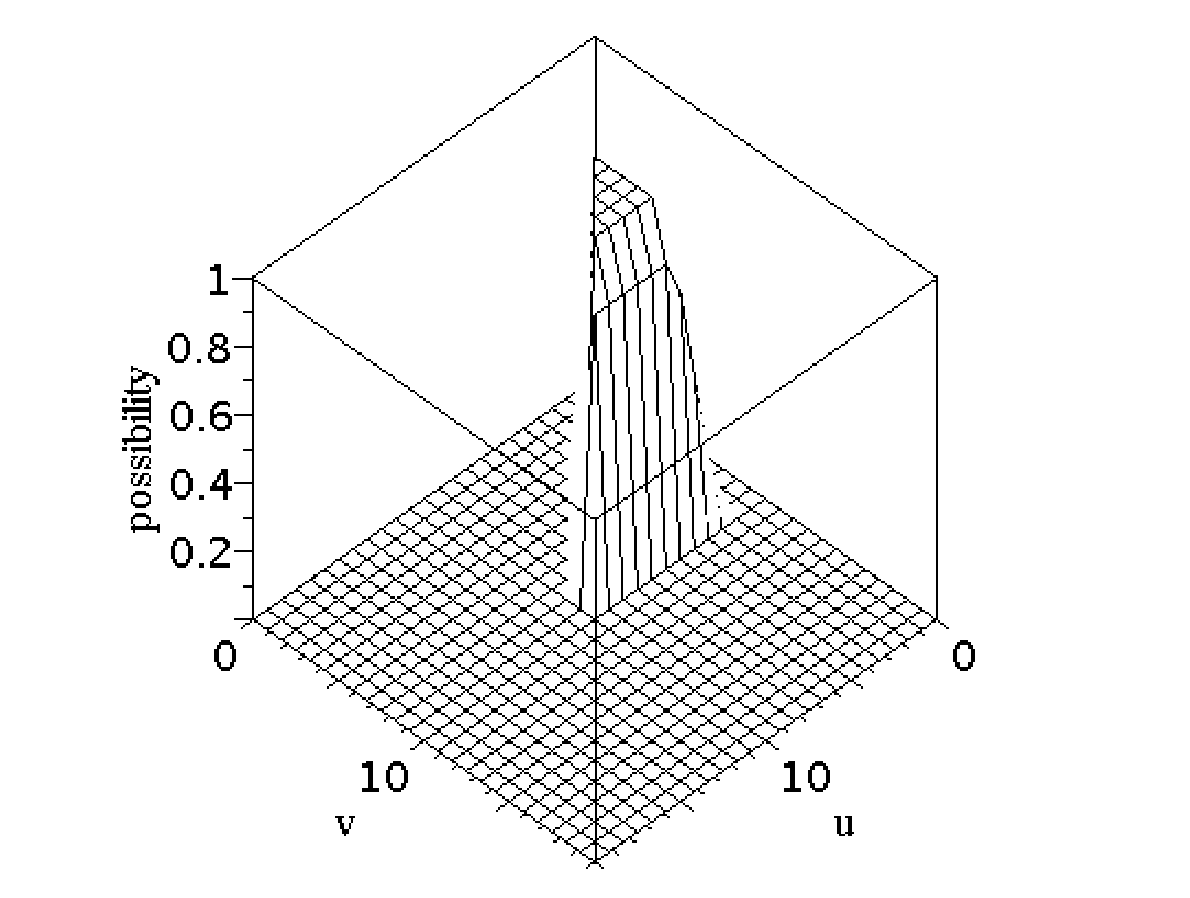
\includegraphics[scale=0.4]{graphs/3D_possibility.eps}
%\caption{Possibility of evaluation for the interval $[a,b]$.}
%\label{fig:3d-possibility}
%\end{figure}
%The necessity plot is obtained in a similar way and is shown in Figure~\ref{fig:3d-necessity}. Notice that the necessity measure is not normalized because the supports of $X$ and $Y$ overlap.
%\begin{figure}[h!]
%\centering
%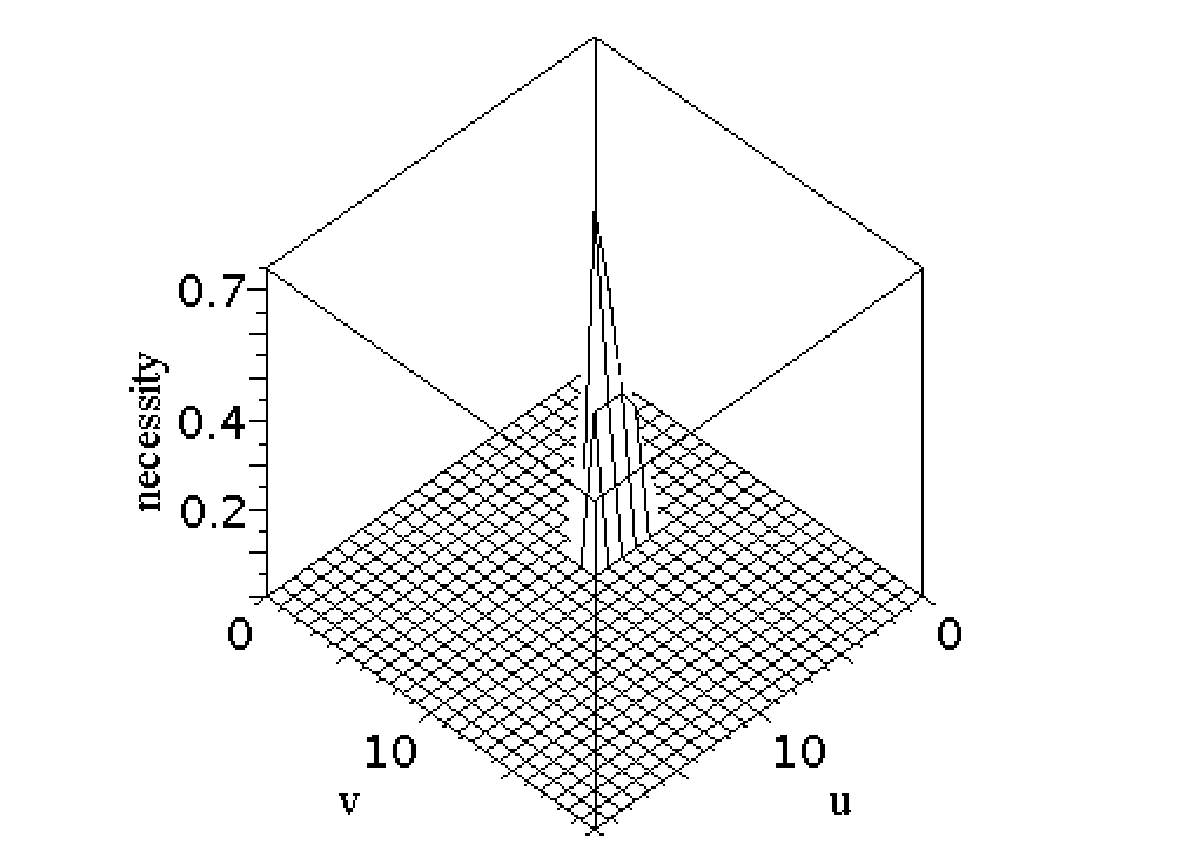
\includegraphics[scale=0.4]{graphs/3D_necessity.eps}
%\caption{Necessity of evaluation for the interval $[a,b]$.}
%\label{fig:3d-necessity}
%\end{figure}



\subsection{Temporal Databases}
%In this section, the proposed reasoning is applied to the specific context of intervals on the real line. This setting is of specific interest in the context of fuzzy temporal databases.
A \emph{temporal database} is a database that manages some aspects of time in its schema. The reality a temporal database tries to model, contains some temporal notions which have to be handled specifically in order to maintain a consistent modelling behavior. A \emph{chronon} is the shortest duration of time supported by the database. Time can be represented either as points or intervals \cite{655777}.
%There are proposals for the fuzzyfication of the time point and the fuzzyfication of the time interval.


%Time granularity is also associated with the representation of the time. A granularity is the result of partitioning on the set of chronons. The conversion among granularities is a common issue within temporal databases \cite{Lin97efficientconversion}. Granularity is the basis of some systems \cite{Cru97},\cite{624013}.

The temporal notions in temporal databases can be classified into 4 types based on their interpretation and modelling purpose. User-defined time has no interpretation, but the other types do:

\begin{itemize}
	\item
	\emph{Transaction time}: The time when the fact is stored in the database.
	\item
	\emph{Valid time}: The time when the fact is true in the modelled reality.
	\item
	\emph{Decision time}: The time when an event was decided to happen. 
\end{itemize}
	
Database models can then be classified into transaction time \cite{Jensen91}, decision time, valid time, bi-temporal \cite{Snodgrass84}(both valid and transaction time) or tri-temporal \cite{Nascimento95} (valid, transaction and decision time) models.


To deal with time points \cite{Dubois89} or intervals \cite{Garrido2009} that are subject to imperfection and can thus not be precisely known, fuzzy temporal models \cite{schockaert08} exist. %Some fuzzy temporal models assume that the time stored in the database is an interval. The temporal interval is represented by two ill-known time points: $X$  an ill-known starting point and $Y$ an ill-known ending point. The interval $\left[X,Y\right]$ is not a fuzzy interval but an ill-known interval: it is a crisp interval but it is partially unknown which values are in this interval.

%%%%%%%%%%%%%%%%%%%%%%%%%%%%%%%%%%%%%%%%%%%%%%%%%%%%%%%%%%%%%%%%%%%%%%%%%
%
% Time
%
%%%%%%%%%%%%%%%%%%%%%%%%%%%%%%%%%%%%%%%%%%%%%%%%%%%%%%%%%%%%%%%%%%%%%%%%%
\subsection{\label{subsec:time-in-databases}Time in Databases}
The concept of time has been studied in databases for a long time. A true standard for adding temporal aspects to relational databases does not exist, but there is a consensus in the literature \cite{Dyreson1994} on what is called a \emph{temporal database}: a temporal database is a database dealing with some aspects of time in its schema.
In a temporal DBMS, a \textbf{chronon} is the shortest duration of time supported by the system. In temporal databases, some temporal attributes can be managed without treating the attribute differently from non-temporal attributes. The time described by such an attribute is called \textbf{user defined time} (\emph{UDT}). In addition to UDT, the following types of time can be discerned in a temporal database, all of which are handled exceptionally by the DBMS:

\begin{itemize}
	\item
	\textbf{Transaction time} (\emph{TT}) \cite{Rowe1987,Jensen1991} denotes the time when the fact (object) is stored in the database. It is usually append-only: as the past cannot be changed, TT cannot be changed either. Furthermore, at the moment of insertion, a TT can be neither in the past nor in the future.
	\item
	\textbf{Valid time} (\emph{VT}) \cite{Jensen1994,Sarda1990,McKenzie1981} denotes the time when the fact (object) is true in the modelled reality. A fuzzy extension has been proposed by \cite{Garrido2009}. 
%	\item
%	User defined time: It is an uninterpreted attribute. The domain is date/time. The query language has no special support for it.
	\item
	\textbf{Decision time} (\emph{DT}) \cite{Nascimento1995,Chakravarthy1994,Etzion1992,Ozsoyoglu1995} denotes the time when an event was decided to happen. 
	\end{itemize}
	
	E.g., consider a database containing employee contract descriptions. The time when the employee's contract is valid, represented by an interval, is VT. The time when the employee's contract is stored in the database is the TT. The time when the decision for hiring this employee was made is the DT.

% is a non-decomposable unit of time.  it  There are two ways to represent a chronon: as a point or as an interval \cite{655777}.

When working with these time concepts, the Data Manipulation Language (\emph{DML}, which is part of the standard database querying language SQL) is extended to deal with possible temporal inconsistencies within the data and to handle more complex (temporal) queries. 
%Next to these concepts, also \textbf{user defined time} (\emph{UDT}) is discerned. UDT is an uninterpreted attribute in the date/time domain. This means that the attribute uses the date/time domain, but the database model does not treat the attribute differently from non-temporal attributes.
Depending on the time managed, a database is classified as either a \textbf{Valid Time Database} (\emph{VTDB}), a \textbf{Transaction Time Database} (\emph{TTDB}), a \textbf{bi-temporal database} (both valid and transaction time are managed) or a \textbf{tri-temporal} or \emph{multitemporal} database (valid time, transaction time and decision time are managed).

%\subsection{Temporal Elements}
%%	
%	In order to define a temporal database model, some basic elements should be defined \cite{Dyreson:1994:CGT:181550.181560}:
%	\begin{itemize}
%	\item A	\textbf{chronon} is a non-decomposable unit of time. In a temporal DBMS, it is the shortest duration of time supported by the system. There are two ways to represent a chronon: as a point or as an interval \cite{655777}.
%	\item
%	\emph{Event}: An instant of time. Usually, an event is said to be occur during time $t$ if it occurs during the chronon represented by $t$.
%	\item
%	\emph{Interval}: The time between two events. The representation is very often a set of contiguous chronons.
	%\item
	%\emph{Span}: A directed duration of time. A duration is an amount of time with known  lenght but no specific starting or ending chronons. The span can be either positive, denoting a forward motion of time or negative, denoting a backward motion of time.
%	\item A	\textbf{timestamp} is a time value associated with some object in the database.	
	
%	\item The	\textbf{lifespan} (of a database object)is the time over which it is defined. The lifespan of a valid time object denotes the time when the corresponding object exists. The lifespan of a transaction time object is the value of the timestamp.
	
	
	
	
	
%	Depending on the type of time the meaning is different:
%		\begin{itemize}
%		\item
%		Lifespan of a valid time object: Refers the time when the corresponding object exists.	
%		\item
%		Lifespan of a transaction time object: The transaction time of a database object refers when the object is stored in the database. The lifespan is the value of the timestamp.		
%		\end{itemize}
%	\end{itemize}
	
%	In the temporal database thesaurus, \emph{'Snapshot'} is the word for non-temporal matters. As a temporal database is a generalization for relational databases, an \emph{snapshot database} is a relational database. Furthermore, a \emph{snapshot relation} is a relation incorporating neither valid nor transaction time.

%\subsection{Main issues when dealing with time}
%Among others, the following problems are present when dealing with time in a database:

%	\begin{itemize}	
%	\item \textbf{Granularity} denotes a partition on the set of chronons. The conversion between several granularities is studied in \cite{Lin97efficientconversion}. Granularity is the base of the temporal model in \cite{Cru97}. An object-oriented implementation is in \cite{624013}.
%	\item	To ensure \textbf{consistency}, temporal databases usually redefine the primary key of a relation. The new primary key takes into account the presence of the time. In order to keep the consistency, the DML is re-defined. For example, in a VTDB, the temporal update sentence is usually composed by an update sentence (closing the old row) plus an insert sentence (creating the new row).
%	\end{itemize}
%Guy's suggestion: instead of imprecision, use imperfection which is more general.
\subsubsection{Imperfection and time}
Representing imprecision and its semantics when dealing with time has been studied for a long time. Several proposals for representing and computing imprecise time indications can be found in \cite{DeCaluwe1997,DeTre1997}. Also, the changes between several granularities can be seen as a source of imprecision \cite{Devos1998}.

In the proposal section we will consider two kinds of imperfection:
\begin{itemize}
\item \textbf{Imperfection in the database} the knowledge about the temporal data contains some imperfection. E.g., a database record shows that \emph{`The car is in the garage around April.'}
 \item \textbf{Imprecision in the query specification} denotes the imprecision in the specification of temporal criteria by the user, when querying. E.g., \emph{`The user wants to obtain a car which is red and which is in the garage around April.'}
\end{itemize}

\subsubsection{Representation}
Several proposals for managing uncertain time in a database exist. Some proposals work with rough sets \cite{Qiang2009}, other proposals rely on possibility distributions for representing uncertainty in time \cite{Dyreson1998,Garrido2009,Galindo2001}. In order to compare temporal possibility distributions, extensions of the classical Allen's operators \cite{Allen1983} are defined in \cite{Ohlbach2004,Nagypal2003,Dubois2003a,Schockaert2008}.
%In the proposal section, we will follow the representation by means of possibility distributions, in order to work with both satisfaction and dissatisfaction degrees. Also, in order to work properly with fuzzy operators, the underlying domain should be numeric. 
% Take a look into this:
%In this paper, the representation for the dates will follow the Julian Day Number (JDN) representation \cite{Dir96}.

%If the starting points and/or the end points of the interval representing the time are not known precisely, it is easy to fuzzify them, using, e.g., two triangular possibility distributions.


In order to deal with uncertainty in time intervals, several proposals are made. Here, two approaches are introduced: the first one, based on \emph{Fuzzy Validity Period}~\cite{Garrido2009} and the second one based on \emph{Possibilistic Valid-time Period}~\cite{JoseEnriquePons2012}.

\begin{definition}
A \textbf{Fuzzy Validity Period} (\emph{FVP}) is defined as a fuzzy time interval specifying when the data regarding an object is valid. A fuzzy time interval is then the fuzzification of a crisp time interval.
\end{definition}
Several options to transform possibility distributions corresponding to the fuzzy starting point and the fuzzy end point into one consistent FVP exist \cite{Garrido2009}, e.g (Fig. \ref{fig:fuzzy-validity-period}):
\begin{itemize}
\item The \textbf{convex hull} approach is the most intuitive approach. The resulting FVP is the convex hull of the union of both fuzzy sets.
\item The \textbf{uncertainty preserving} approach is less intuitive but more realistic. The amount of uncertainty is maintained at the edges of the possibility distribution representing the FVP \cite{Garrido2009}.
\end{itemize}

%%%%%%
% FUZZY VALIDITY PERIOD
%%%%%%
\vspace*{13pt}
\begin{center}
{
\includegraphics[scale=0.25]{./graphs/comparisoncv.pdf}

}
\end{center}
%\centerline{ 
\psfig{file=./graphs/Y-time-point.eps}}
\vspace*{10pt}
\fcaption{\label{fig:fuzzy-validity-period}Transformation to obtain the FVP. The top graph shows the two triangular possibility distributions. The middle graph shows the convex hull validity period, the bottom one shows the result of the second transformation, which maintains the imprecision.}
%  \label{fig:fuzzy-validity-period}
\vspace*{13pt}

\begin{definition}
A \textbf{Possibilistic Valid-time Period} (\emph{PVP}) is an ill-known interval in time specifying when the data regarding an object is valid.
\end{definition}
A PVP is an ill-known interval in the sense of definition \ref{def;possibilistic-variable}, section \ref{subsec:possibilistic-variables}. Note that this representation is \emph{disjunctive}: the PVP represents only one crisp time interval, but that for some reason it is (partially) unknown.

The ill-known interval approach has many advantages from the representation by the FVP as demonstrated in \cite{Pons2011},\cite{Pons2012}. Table \ref{tbl:comparative-pvp-fvp} is a comparative between PVP and FVP. The following list defines the items in the comparative:

\begin{enumerate}
\item Domain: The domain of the possibility distribution modelled by the approach.
\item Implementation of relationships: How to implement a relationship.
\item Allen's relations: Are the Allen's relations defined?
\item Storage: The way the data is stored in the database.
\item Possibility measures: Does the framework provides always a possibility measure for any relation between the temporal elements?
\item Necessity measures:  Does the framework provides always a necessity measure for any relation between the temporal elements?
\end{enumerate}


%%
%% comparison table between pvp and fvp.
%%
\vglue13pt
%\begin{table}[htbp]
\tcap{Comparative PVP vs FVP}
%\centerline{\small DATA TYPES}
\vglue-6pt
\centerline{\small\baselineskip=13pt
\begin{tabular}{c p{2cm} p{2cm}}\\
Item & PVP & FVP\\
\hline
(1) & $\Pow(\R)$ & $\R$ \\
(2) & Ill-known constraints. & Ad-hoc operators. \\
(3) & $\checkmark$ & - \\
(4) & Two distributions one for each endpoint. & Only one distribution. \\ 
(5) & $\checkmark$ & $\checkmark$ \\
(6) & $\checkmark$ & - \\
\hline\\
\end{tabular}
\label{tbl:comparative-pvp-fvp}
} 

In the rest of the paper we will work only with PVP to represent valid-time intervals.


\subsection{\label{subsubsec:Understanding-valid-time-databases}Understanding Valid-time Databases}
This subsection is devoted to describe the behaviour of a crisp valid-time database. For the shake of simplicity, only the three main operations in the Data Manipulation Language \emph{DML} a.k.a \emph{CRUD} (CReate Update, Delete) operations are shown. Usually the DML operations in a temporal database are re-defined e.g. a typical update sentence in SQL could be re-defined by means of several insert and update sentences. Therefore, in order to be clear, these high level primitives in the DML for a valid-time database are usually noted as Insert, Modify and Delete. In the following subsections each primitive is defined and explained. Finally a illustrative example is given. For a more complete information on the behaviour of a bitemporal database, please refer to ~\cite{Jensen1994}.

\begin{definition}
Consider a relation $R$ in a temporal database, an entity $A$ given by the attributes $\left(a_1, \ldots, a_n \right)$ and the crisp time interval $I$ given by $\left[a,\ b\right] : a,b \in \T, a \leq b$. The pair $\left(A, I\right)$ expresses that the data regarding the entity A is valid during the crisp time interval I.  Note that the relation $R = \left(A, I \right) x \left(A, I \right)$. The following equation indicates that the pair $\left(A, I\right)$ is in the relation R:
\begin{equation}
\label{eq:rel-def}
\left( R, \left(A , I\right) \right)
\end{equation}
\end{definition}
\begin{example}
\label{ex:library-database}
 Consider a library database. Each physical book is stored with an identifier (ID), a title and the start and end loan dates respectively. Table \ref{tbl:library-sample} illustrates the first version of the database, after three insertions. In this example, $A = ($ ID, Title $)$ and $I = ($ Start Loan, End Loan $)$.
\end{example}





\vglue13pt
%\begin{table}[htbp]
\tcap{\label{tbl:library-sample}Sample library database}
\centerline{\small DATA TYPES}
\vglue-6pt
\centerline{\small\baselineskip=13pt
\begin{tabular}{c c c c}\\
\hline
\textbf{ID}  & Title  & Start Loan & End Loan \\
\hline
3 & Dracula & 15/3/2012 & 30/3/2012 \\
4 & Frankenstein & 25/3/2012 & 4/4/2012 \\
5 & Harry Potter & 18/3/2012 & 2/4/2012\\
3 & Dracula & 4/4/2012 & UC \\
\hline\\
\end{tabular}
}

In order to simplify the algorithms for the manipulation of data, some auxiliary functions and constants are defined:

\begin{definition}
 \label{def:until-changed}
\textbf{Until changed (UC):} To show that the data related to the entity $\left(A, I \right)$ is up-to-date, a special constant called \emph{Until Changed} is defined for the endpoint, $d$, of the time interval $I = \left(c, d\right)$. The value for this constant is considered to be $+\infty$. 
\end{definition}



If the pair $\left(A, I \right)$ with $I = \left(c, UC \right), c \in \T$ is in the relation $R$, then, it is said that the pair $\left(A, I \right)$ is \emph{current} in the relation.

For example, last row in Table \ref{tbl:library-sample}. The value for the time interval is $I = \left(4/4/2012 , UC \right)$. The meaning is that the book with ID = 3 was loaned the  4/4/2012 and it is still loaned. The book with ID = 3 is current in the relation.

\begin{definition}
\textbf{Current $\left(R, A \right)$:}
\label{def:current-in-relation}
This function returns a crisp time interval $I$ if the entity $A$ is current in the relation $R$ or the empty set, if the entity $A$ is not current in the relation.

%Consider an object $A$ and a relation $R$ in a temporal database. The function Current$\left(R, A \right)$ obtains the tuple $\left(A, I \right)$ that is current in the relation $R$, that is it, $I = \left[a, +\infty \right]$.

\begin{align}
\label{eq:current-in-relation}
\mbox{Current} \left(R, A \right) &=& \\ 
\begin{cases}
\nonumber
I & \mbox{ if } (A,I) \in R \wedge I = \left(c, UC \right), c \in \T\\
\emptyset & \mbox{ in any other case }
\end{cases}
\end{align}
\end{definition}

For example, the function Current(R, (3,`Dracula')) returns the time interval $I = \left(4/4/2012 , UC  \right)$. On the other hand, Current(R, (4,`Frankenstein')) returns the empty set.

The following two Allen's relations (see Figure \ref{fig:allen-rel}) are defined~\cite{Nagypal2003} to implement the auxiliary functions. 



\vspace*{13pt}
\begin{center}
{
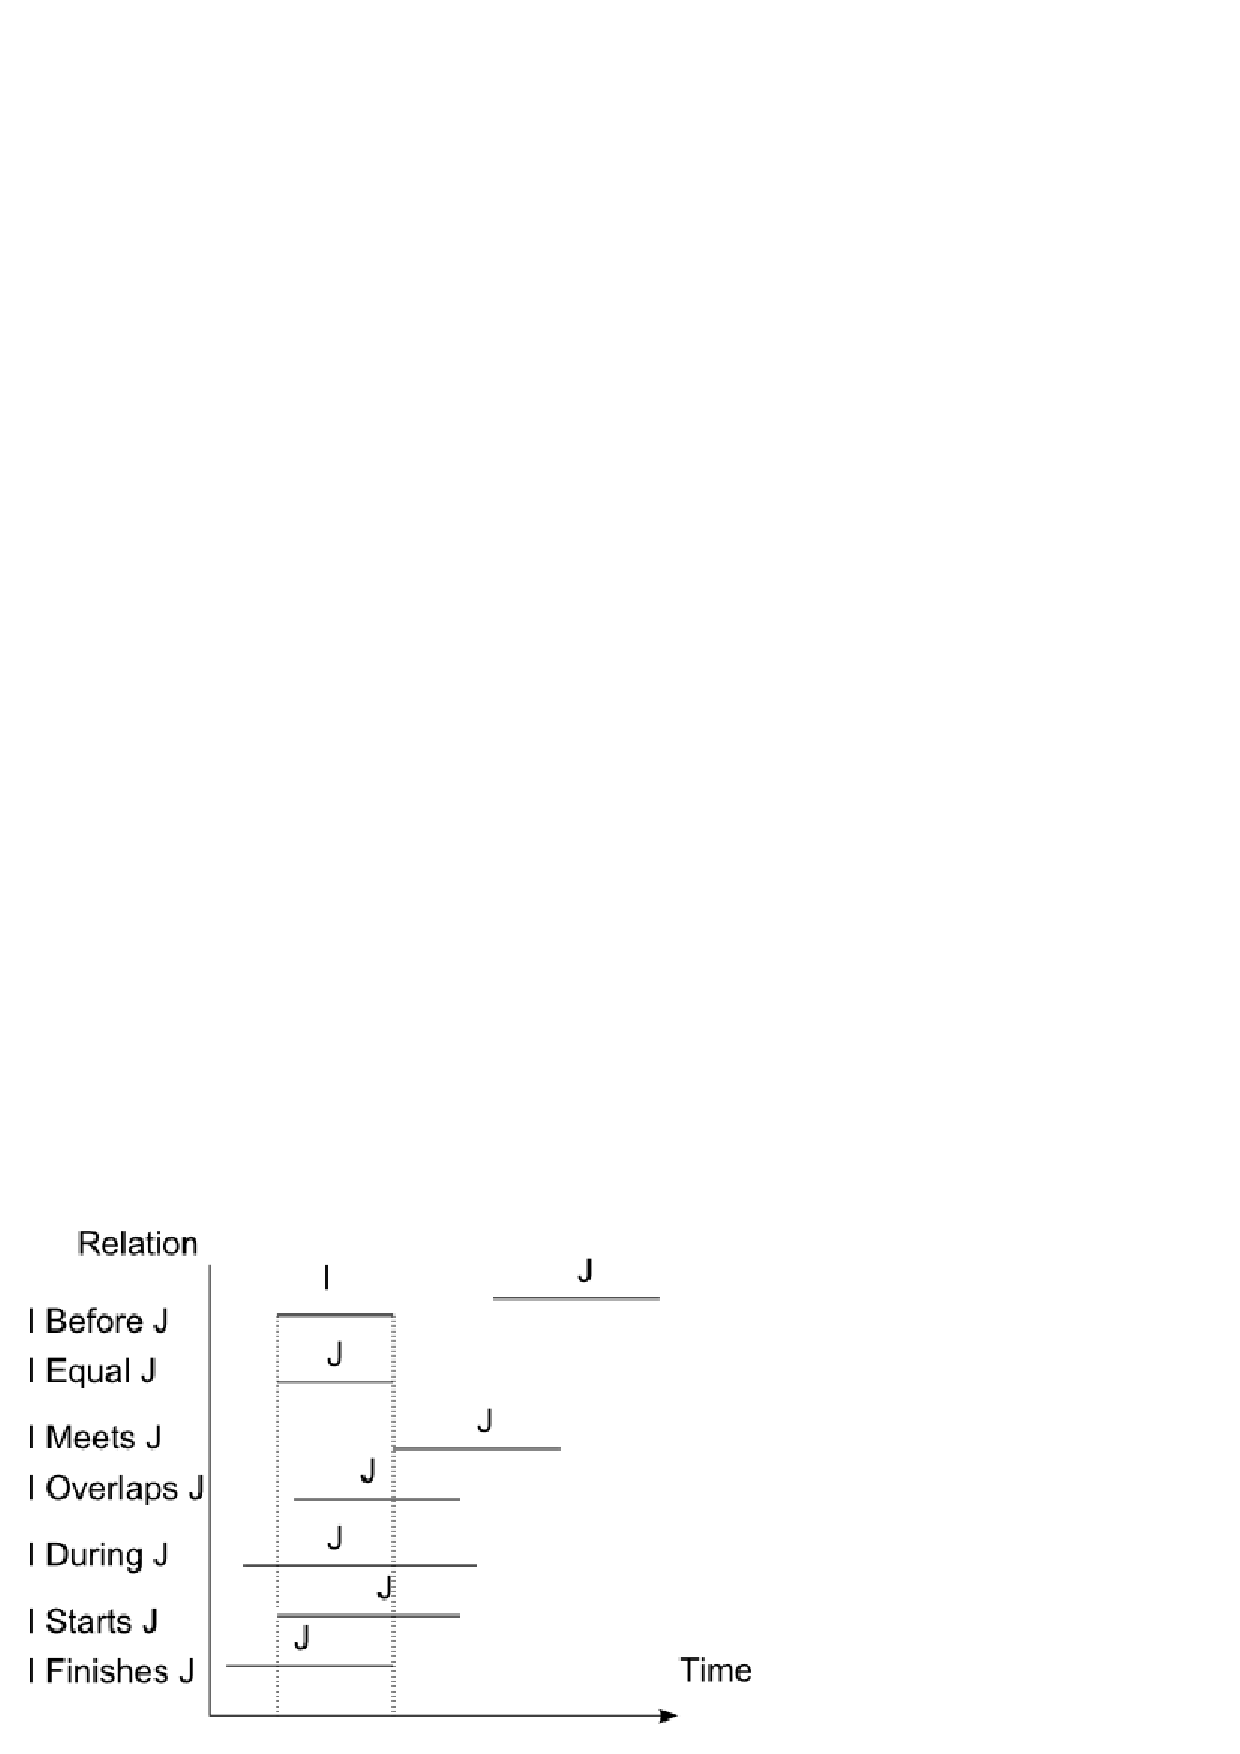
\includegraphics[scale=0.5]{./graphs/allen.pdf}

}
\end{center}
%\centerline{ 
\psfig{file=./graphs/Y-time-point.eps}}
\vspace*{10pt}
\fcaption{\label{fig:allen-rel}Allen's relations for two crisp time intervals $I$ and $J$.}
\vspace*{13pt}


\begin{definition}
\textbf{Overlaps:}
 \label{def:overlaps}
Given two time intervals $I = \left(c, d \right)$ and $J = \left(e, f\right)$, it is said that I overlaps J if:
\begin{equation}
 \label{eqn:overlaps}
\text{I Overlaps J}  = \left(c > e  \right) \wedge \left(d < f  \right) 
\end{equation}
\end{definition}
  

\begin{definition}
\textbf{During:}
 \label{def:during}
Given two time intervals $I = \left(c, d \right)$ and $J = \left(e, f\right)$, it is said that I during J if:
\begin{equation}
 \label{eqn:during}
\text{I During J}  = \left(c < e  \right) \wedge \left(d > e  \right) \wedge \left(d < f \right)
\end{equation}
\end{definition}

\begin{definition}
\textbf{CloseR$\left( I, J \right)$:}
\label{def:close-a-crisp-interval-r}
Consider two crisp intervals $I= \left[c ,d \right]$ and $J= \left[e ,f \right]$. The CloseR$\left(I, J\right)$ function allows to close the right-open interval $I$ with respect to the first value $e$ in $J$:
\begin{align}
\label{eq:close-a-crisp-interval}
\mbox{CloseR} \left( I, J \right) &=& \\ 
\begin{cases}
\nonumber
%I & \mbox{ if } b \neq +\infty \\
%I=\left[a, c \right[ & \mbox{ if } b = +\infty \wedge J > I
\left[c, e \right[ & \mbox{ if } d = UC \wedge J \mbox{ During } I \\
I & \mbox{ in any other case.}
\end{cases}
\end{align}
\end{definition}

For example, consider two time intervals, $I = \left(4/4/2012, UC \right)$ and $J = \left(24/4/2012, UC \right)$. The result of applying the CloseR$\left(I, J \right)$ is $I = \left(4/4/2012, 23/4/2012 \right)$.




%Analogously, it is defined the function to close a left-open interval: 
%\begin{definition}
%\label{def:close-a-crisp-interval-l}
%CloseL$\left(I, J\right)$ 
%\begin{align}
%\mbox{CloseL} \left( I, J \right) &=& \\ 
%\begin{cases}
%\nonumber
%I & \mbox{ if } a \neq -\infty \\
%I=\left]d, b \right] & \mbox{ if } a = -\infty \wedge J < I
%\end{cases}
%\end{align}
%\end{definition}




%\begin{definition}
%\label{def:first-in-relation}
%Analogously, the function First$\left(R, A \right)$ obtains the tuple $\left(A, I \right)$ where $I$ is a right-open interval and which is the first version in the relation $R$, that is it, $I = \left[-\infty, b \right]$.
%\begin{align}
%\label{eq:first-in-relation}
%\mbox{First} \left(R, A \right) &=& \\ 
%\begin{cases}
%\nonumber
%I & \mbox{ if } \exists b \in I : (A,I) \in R \wedge a = -\infty \\
%\emptyset & \mbox{ in any other case }
%\end{cases}
%\end{align}
%
%\end{definition}



Now it is possible to close the current version of an entity by using \eqref{eq:close-a-crisp-interval} and \eqref{eq:current-in-relation}. This functionality is required to append new information about an existing entity in the relation.

\begin{definition}
\label{def:close-current-version}
Consider an entity $A$, the relation $R$ and a time interval $J$. Then, the function close-current$\left(R,\left(A,J\right) \right)$ closes any current version of the object $A$ if it exists and add the new version $\left(A, J \right)$.

\begin{eqnarray}
\label{eq:close-current}
\text{Close-current} \left(R, \left(A, J\right) \right) =\\
\begin{cases}
\nonumber
R - \left(A, I \right) \cup \left \lbrace \left(A, \mbox{ CloseR } \left(I, J\right) \right)\right \rbrace \cup \left \lbrace\left(A, J\right) \right \rbrace  \\
\nonumber
\mbox{ if } I = \mbox{ Current } \left(R, A \right)\\ %\wedge J > \mbox{ CloseR } \left(I, J \right)   \\
\nonumber R , \text{ in any other case}
\end{cases}
\end{eqnarray}
\end{definition}

For example, consider the book with ID = 3 in Table \ref{tbl:library-sample}. The current version was loaned on 4/4/2012. The book was returned to the library but, for some reason, the end loan date was not registered. The book is loaned again on 24/4/2012. Then, the Close-current function allows to close the current version of the book and insert a new version. First, the function CloseR is applied with $I = \left(4/4/2012, UC \right)$ and $J = \left(24/4/2012, UC \right)$. Hence, the value for the time interval $I$ is $ \left(4/4/2012, 23/4/2012 \right)$. Then, the modifications on the value for the time interval $I$ are stored. Finally, a new row with the current values of the book and the time interval $J$ is stored.
The result of this operation is illustrated on Table \ref{tbl:library-sample-2}.




%It is also possible to append at the beggining by using \eqref{def:close-a-crisp-interval-l} and \eqref{def:first-in-relation}.
%\begin{definition}
%\label{def:append-first-version}
%Consider an object $A$, the relation $R$ and a time interval $J$. Then, the function append-first$\left(R,A,J \right)$ closes any right open version of the object $A$ if it exists and add the new version $\left(A, J \right)$.
%
%\begin{eqnarray}
%%\label{eq:close-current}
%\text{Append-first} \left(R, A, J \right) =\\
%\begin{cases}
%\nonumber
%\big \lbrace R - \left(A, I \right) \cup \left \lbrace \left(A, \mbox{ CloseL } \left(I, J\right) \right) \cup \left(A, J\right)\right \rbrace  \big \rbrace \\
%\nonumber
%\mbox{ if } I = \mbox{ First } \left(R, A \right) \wedge J < \mbox{ CloseL } \left(I, J \right)   \\
%\nonumber R , \text{ in any other case}
%\end{cases}
%\end{eqnarray}
%\end{definition}
\subsubsection{\label{subsubsec:modify}Modify}
This operation adds new information about an existing entity $A$ in the relation $R$. The modify operation does not remove any previous value of the object $A$. It closes the current version for the entity $A$ and adds a new version.


%Note that the modify operation is only applicable when the object $A$ is current in the relation $R$; $ \left(A, I \right) \in R, I = \left[a, +\infty \right]$.

\begin{align}
\label{eq:modify}
\MOD \left( R, \left(A, I \right)\right) =\\
%\begin{cases}
\nonumber
\mbox{ Close-current }\left(R, \left(A, I\right) \right) %\\
% \mbox{ if Current}\left(R ,A \right) \neq \emptyset \\
% R,  \mbox{ otherwise }
%\end{cases}
\end{align}


\subsubsection{\label{subsubsec:insert}Insert}
The user wants to store an object $A$ which is valid in the relation $R$ during the time interval specified by $I = \left(a, b \right)$.
%
%
%The interpretation of the insert operation is the following: The user wants to store in the database that an object $A$  is true for some period(s) of time $I$ in the given relation $R$. To indicate that the object $A$ is current in the relation, the special value Until Current, $\UC$  is used. 
There are two main cases when performing a create operation:
\begin{enumerate}
\item The object $A$ was never in the relation $R$: The object is added with the valid-time indicated by the crisp interval $I$. In the example, this correspond with the following insertion sentences:
\begin{verbatim}
Insert(3,'Dracula',
(15/3/2012, 30/3/2012));
Insert(4,'Frankenstein',
(25/3/2012, 4/4/2012));
Insert(5,'Harry Potter',
(18/3/2012, 2/4/2012));
\end{verbatim}


\item The object $A$ is in the relation $R$. Depending on the value of the time interval $I$, there are three possibilities:
	\begin{enumerate}
	\item Insert $\left(A, I\right)$ in the relation $R$. If the time interval $I$ does not overlap any other valid-time interval in the relation $R$. For example, consider that the book with ID 3 is loaned on 4/4/2012 but the book has not been returned yet. This is illustrated in Table \ref{tbl:library-sample}. The insert sentence is:
	      \begin{verbatim}
Insert(3,'Dracula',
(4/4/2012, UC));
	      \end{verbatim}


	\item Modify and close the current version of $A$ and insert $\left(A, I\right)$. For example, consider now that the book with ID 3 is loaned  the 24/4/2012. Here the problem is that the book with ID 3 was loaned on 4/4/2012, but not returned. If the book is already in the library for a new loan, then it is necessary to set the return date and add a new row with the new loan date. This is illustrated in Table \ref{tbl:library-sample-2}, the insert sentence is:
	    \begin{verbatim}
Insert(3,'Dracula',
(24/4/2012, UC));
	      \end{verbatim}
	\item Reject the insertion, if the time interval $I$ does overlap any existing valid-time interval for the object $A$ in the relation $R$. For example, consider now that the librarian wants to introduce a past loan for the book with ID 3. The book was loaned on 6/4/12/2012 and returned on 25/4/2012. As this interval does overlaps other time intervals, it is not possible that the book was loaned in that time interval.Therefore, the insertion is rejected. The insert sentence is:

	      \begin{verbatim}
Insert(3,'Dracula',
(6/4/12/2012,25/4/2012));
	    \end{verbatim}


	\end{enumerate}

\end{enumerate}

\vglue13pt
%\begin{table}[htbp]
\tcap{\label{tbl:library-sample-2}Sample library database}
%\centerline{\small DATA TYPES}
\vglue-6pt
\centerline{\small\baselineskip=13pt
\begin{tabular}{c c c c}\\
\hline
\textbf{ID}  & Title  & Start Loan & End Loan \\
\hline
3 & Dracula & 15/3/2012 & 30/3/2012 \\
4 & Frankenstein & 25/3/2012 & 4/4/2012 \\
5 & Harry Potter & 18/3/2012 & 2/4/2012\\
3 & Dracula & 4/4/2012 & 23/4/2012 \\
3 & Dracula & 24/4/2012 & UC \\
\hline\\
\end{tabular}
}



The algorithm for the implementation of the insert operation is the following:

\begin{align}
\label{eq:insert}
\INS \left(R ,\left(A, I\right)\right) =\\
\begin{cases}
\nonumber
R \cup \left(A, I \right) & \mbox{ if }  (A, I ) \not \in R  \vee \\
 &   \left(A, J\right) \in R \wedge \lnot \left(I \mbox{ Overlaps } J\right) \\
\mbox{modify(R,(A,I))} & \mbox{ otherwise }    %\mbox{ if } \exists J \left(A,J\right) \in R \wedge \mbox{Current(A,J)} \\ 
%R, &   
\end{cases} 	
\end{align}

\subsubsection{\label{subsubsec:del}Delete}
The delete operation logically removes a current entity $A$ which is valid in the relation $R$:
\begin{align}
\label{eq:delete}
\DEL \left(R ,A \right) =\\
\begin{cases}
\nonumber
R - \left(A, I \right), & \forall \left( A, I \right) \in R\\
R, & \mbox{ otherwise }  
\end{cases} 	
\end{align}

For example, consider that the librarian wants to delete the history for the book with ID = 3. The result of this operation is shown in Table \ref{tbl:library-sample-3}. The delete sentence is:

\begin{verbatim}
 Delete(3,'Dracula');
\end{verbatim}


\vglue13pt
%\begin{table}[htbp]
\tcap{\label{tbl:library-sample-3}Sample library database}
%\centerline{\small DATA TYPES}
\vglue-6pt
\centerline{\small\baselineskip=13pt
\begin{tabular}{c c c c}\\
\hline
\textbf{ID}  & Title  & Start Loan & End Loan \\
\hline
4 & Frankenstein & 25/3/2012 & 4/4/2012 \\
5 & Harry Potter IV & 18/3/2012 & 2/4/2012\\
\hline\\
\end{tabular}
}


\subsubsection{\label{subsubsec:revise}Revise}
This operation replaces the old values for the entity $A'= \left(a_1', \ldots, a_n' \right) $ with the new values specified by $A = \left(a_1, \ldots, a_n \right)$ in the relation $R$, at a given time interval $I$. This operation is used when a correction on the values for the entity $A$ should be done.
\begin{align}
\REV\left(R, \left(A, I \right) \right)=\\
\begin{cases}
\nonumber
 R - \left(A', I \right) \cup \left \lbrace \left(A, I \right) \right \rbrace & \mbox{ if } \left(A', I \right) \in R  \\
   %: A = \left(a_1, \ldots, a_n \right),\\
%A'= \left(a_1', \ldots, a_n' \right)   \\   
R & \mbox{ otherwise }
\end{cases}
\end{align} 

For example, consider now that the librarian wants to make a correction in the title for the book with ID = 5. The new title is `Harry Potter IV'. The result of this operation is illustrated in Table \ref{tbl:library-sample-3}.
 Then, the revise sentence is:

\begin{verbatim}
Revise(5,'Harry Potter IV', 
(18/3/2012, 2/4/2012));
\end{verbatim}




\section{\label{sec:time-rep}Time representation}
%%%%%%%%%%%%%%%%%%%%%%%%%%%%%%%%%%%%%%%%%%%%%%%%%%%%%%%%%%%%%%%
%
% Time representation
%
%%%%%%%%%%%%%%%%%%%%%%%%%%%%%%%%%%%%%%%%%%%%%%%%%%%%%%%%%%%%%%%%

This section is devoted to specify the representation of time within the framework of the possibility theory. First of all, the specification for a single ill-known temporal point shall be explained. Then, the formal specification and the related constraints are given for an ill-known valid-time interval.

\subsection{\label{subsec:ill-known-point-rep}Ill-known time point}
An ill-known time point $X$ is a precise time point that, for some reason, it is not fully specified. Note that $X$ has only one possible value but that value is unspecified.

\begin{definition}
\label{def:ill-known-time-point}
\textbf{Ill-known time point.}\\
Consider a time domain $\T$, uncertainty about the values of the ill-known time point $X$ is given by the possibility distribution $\pi_X$:
\begin{equation}
\label{eq:ill-known-time-point}
\Pi(X) = \pi_X(t) \in \left[0,1\right] , t \in \T
\end{equation}
\end{definition}

It is also possible to specify an ill-known time point by a convex combination of ill-known constraints, (Definition \ref{def:convex-combination-ill-known-constraints}) as shown by equation \eqref{eq:ill-known-value-def-by-const-unc}.



\begin{definition}
\label{def:ill-known-domain}
\textbf{Domain for an ill-known time point.}\\
Consider $\Pow(\T)$ the set of all the possibility distributions over $\T$, and the three fuzzy constants \emph{UNKNOWN} $=\left\lbrace 1/t, \forall t \in \T \right\rbrace$, \emph{UNDEFINED} $=\left\lbrace 0/t,\forall t \in \T \right\rbrace$ and \emph{NULL} $=\lbrace 1/$ \emph{UNKNOWN}, $1/$ \emph{UNDEFINED} $\rbrace$. The domain for an ill-known time point $X$ is given by: 
\begin{align}
\label{eq:ill-known-domain}
\Dom (X) =  \lbrace \Pow(\T) & \cup \mbox{\emph{UNKNOWN}} \\
\nonumber
&\cup \mbox{\emph{UNDEFINED}} \\
\nonumber
&\cup \mbox{\emph{NULL}} \rbrace
%
\end{align}
\end{definition}




\subsubsection{\label{subsubsec:ill-known-time-datatypes}Datatypes}
The data type for the representation of an ill-known time point allows the representation of the values shown in Table \ref{tbl:time-point-types}
%The datatypes for an  $X$ are shown in Table \ref{}.
\vglue13pt
%\begin{table}[htbp]
\tcap{\label{tbl:time-point-types}Values for the time point data type.}
\centerline{\small TIME POINT DATA TYPE}
\vglue-6pt
\centerline{\small\baselineskip=13pt
\begin{tabular}{c p{0.4\columnwidth} p{0.3\columnwidth}}\\
Subtype & Value & Representation \\
\hline
1 & A single time point &  $1/x, x \in \T$\\
2 & A possibility distribution in the numeric domain & A fuzzy number or a fuzzy interval.\\
3 & An unknown value & \textbf{UNKNOWN}$= \lbrace1/t,\forall t \in \T \rbrace$\\
4 & An undefined value & \textbf{UNDEFINED}$= \lbrace 0/t,\forall t \in \T \rbrace$\\
5 & A null value & \textbf{NULL} $=\lbrace 1/$Unknown, 1/Undefined $\rbrace$\\
\hline\\
\end{tabular}
}

%Example of different uses of the ill-known time value.
\begin{example}
Consider a historical database with data from diplomatic documents. The following fields are stored: the digital identifier \emph{ID} which is the primary key  and the estimated time when the document was sent (field \emph{Date}). Table \ref{tbl:sample-time-point} contains some example data from this database. 
\end{example}

\vglue13pt
%\begin{table}[htbp]
\tcap{Sample of the historical database}
%\centerline{\small DATA TYPES}
\vglue-6pt
\centerline{\small\baselineskip=13pt
\begin{tabular}{c c}\\
\textbf{ID} & Date\\
\hline
23454 & Unknown \\ 
34563 & 11/12/1204 \\
12211 & $\left[7/2/1204,30,30\right]$ \\
23455 & $\left[10,10/6/1204,20/6/1204,15 \right]$ \\
\hline\\
\end{tabular}
\label{tbl:sample-time-point}
} 
 
In that database, for the document with ID=23454, all the dates in the domain are equally possible. Nevertheless, the document 34563 was sent in the crisp (exact) date 11/12/1204. The time for documents 12211 and 23455 are specified with several possibility distributions. The first one is also known as a fuzzy number whereas the second one is also known as a fuzzy interval, as explained in Section \ref{sec:prelim}.
 
%\end{example}
 
 


\subsection{\label{subsec:ill-known-interval}Ill-known time interval}


\begin{definition}
\textbf{Ill-known time interval}\\
An ill-known time interval denoted by $\left[X, Y\right]$ is a precise time interval whose boundaries are not precisely known. The ill-known interval is defined by two ill-known points, namely $X$,$Y$.
In order to know if all the points in the crisp time interval $I=\left[a, b\right]$ are within the boundaries of the ill-known time interval $\left[X, Y\right]$ we define the following two ill-known constraints $C_{1}, C_{2}$ 
\begin{eqnarray}
\label{eq:constraint-c1}
C_1\stackrel{\triangle}{=}\left(\geq,X\right)  \\
\label{eq:constraint-c2}
C_2\stackrel{\triangle}{=}\left(\leq,Y\right)
\end{eqnarray}
Note that the boolean operator applied to the constraints is $\bool=\wedge$. Hence, the construct of both constraints is $C_1 \wedge C_2$
This means that we want to know if all the points in the interval $I$ are greater or equal to $X$ and, at the same time, smaller or equal to $Y$.
\end{definition}

%% equations for the poss and nec!!
The simplified equations for the possibility and the necessity measures are~\cite{Pons2011}:
\begin{eqnarray}
\label{eq:interval-pos}
\Pos\left(\lambda([a,b])\right)&=&\\
\nonumber
\min\bigg(\sup_{a\leq w}\pi_{X}(w),\sup_{b\geq w}\pi_{Y}(w)\bigg)\\
\label{eq:interval-nec}
\Nec\left(\lambda([a,b])\right)&=&\\
\nonumber
\min\bigg(\inf_{a>w}1-\pi_{X}(w),\inf_{b<w}1-\pi_{Y}(w)\bigg).
\end{eqnarray}




\subsubsection{\label{subsubsec:open-interval}Open ill-known time intervals}
Quite often, the user may want to specify time intervals with open boundaries in one or both endpoints. Consider an ill-known time interval $\left[X, Y\right]$. Then it is possible to distinguish between the following two types of open intervals:
%\begin{enumerate}
%\item
\begin{definition}
\textbf{Completely unknown time interval}: Both starting and ending points are unknown, therefore the whole interval is unknown.
%specified by the \emph{UNKNOWN} constant. Due to the representation, both endpoints, say $X$ and $Y$, are stored. Thus, the interval is stored as $[$ \emph{UNKNOWN}, \emph{UNKNOWN} $]$. 
\end{definition}

%\item
\begin{definition}
\textbf{Semi-open time interval}: Only one of the two ill-known endpoints for the time interval $\left[X, Y\right]$ is unknown. Example \ref{ex:open-time-interval} and Figure \ref{fig:example-open-time-interval} illustrates a left open time interval.
% Note that due to the ill-known constraints $C_{1}, C_{2}$ it is not possible a representation like $[$ \emph{UNKNOWN} $, Y]$ or $[X, $ \emph{UNKNOWN} $]$. The solution adopted for this problem is explained in the following paragraph. 
\end{definition}
%\end{enumerate}

\subsubsection{\label{subsubsec:representation-semi-open}Representation of semi-open time intervals}
As mentioned before, the problem resides in the representation of these kind of interval. In order to get a short representation for these intervals, two constants are defined: $FB$ \emph{From the Beginning}: it is only valid for the left value of the interval and $UC$ \emph{Until Changed} (this name is usual in the temporal database community, see ~\cite{Jensen1994}) which is only valid for the right value of the interval. Note that these two constants are aliases for a function that obtains both possibility and necessity measures. 

Because of the ill-known constraints $C_{1}, C_{2}$, a function called \emph{Open} should be defined in order to deal with a proper representation of these intervals:

\begin{definition}
\label{def:open-func}
$Open(C)$\\
The function $\Open(C)$ provides both possibility and necessity measures for all the points in the open part of a semi-open ill-known time interval.
The parameter $C$ is an ill-known constraint $C\stackrel{\triangle}{=}\left(R,T\right)$ as defined in \ref{subsec:interval-evaluation-by-ill-known-constraints}, in the equation \eqref{eq:ill-known-constraint} and in~\cite{Pons2011}.
The possibility and necessity measures are defined by:
\begin{eqnarray}
\label{eq:open-pos-nec}
\Pos\left(\Open(C)\right) &=& \Big(\sup_{r\in\T \Rp\  w}\pi_{T}(w)\Big)\\
\Nec\left(\Open(C)\right) &=& \Big(\inf_{r\in\T \Rn\  w}1-\pi_{T}(w)\Big)
\end{eqnarray}
Where the values for the binary relations $\Rp$ and $\Rn$ are shown in Table \ref{tbl:open-pos-nec-rels}.
\end{definition} 

\vglue13pt
%\begin{table}[htbp]
\tcap{Relations for the $\Open(C)$ function. Depending on the relation $R = \left(\leq, <, >, \geq\right)$ in the constraint $C$, the values for $\Rp$ and $\Rn$ are shown.}
\centerline{\small Relations}
\vglue-6pt
\centerline{\small\baselineskip=13pt
\begin{tabular}{c c c}\\
\hline
Constraint & $\Rp$ & $\Rn$\\ \hline
$C\stackrel{\triangle}{=}\left(<,T\right)$ & $>$ & $\leq$ \\
$C\stackrel{\triangle}{=}\left(\leq,T\right)$ & $\geq$ & $<$ \\
$C\stackrel{\triangle}{=}\left(>,T\right)$ & $<$ & $\geq$ \\
$C\stackrel{\triangle}{=}\left(\geq,T\right)$ & $\leq$ & $>$ \\
\hline\\
\end{tabular}
\label{tbl:open-pos-nec-rels}
}

As explained before, the constants $\FB$ and $\UC$ are aliases for the function $\Open$ with the following parameters:
\begin{eqnarray}
\FB &=& \Open(C_2)\\
\UC &=& \Open(C_1)
\end{eqnarray}

Where the constraints $C_1$ and $C_2$ are given in equations \eqref{eq:constraint-c1} and \eqref{eq:constraint-c2}.

\begin{example}
\label{ex:open-time-interval}
Consider an ill-known time interval given by $\left[\FB, Y \right]$. Consider also that in this case, $Y= \left[15/10/2012,3,4 \right] $. Figure \ref{fig:example-open-time-interval} shows the representation for $Y$. The user wants to obtain the possibility and the necessity measures for the $\FB$ part of the interval are:
\end{example}

\begin{eqnarray}
\nonumber
\FB = \Open(C_2) \mbox{ with } C_2\stackrel{\triangle}{=}\left(\leq,Y\right)\\
\nonumber
\Pos\left(\Open(C)\right) = \Big(\sup_{r\in\T \geq\  w}\pi_{Y}(w)\Big)\\
\nonumber
\Nec\left(\Open(C)\right) = \Big(\inf_{r\in\T <\  w}1-\pi_{Y}(w)\Big)
\end{eqnarray}


\vspace*{13pt}
\begin{center}
{

\includegraphics[scale=1]{./graphs/open-time-interval.pdf}
\label{fig:example-open-time-interval}
}
\end{center}
%\centerline{ 
\psfig{file=./graphs/Y-time-point.eps}}
\vspace*{10pt}
\fcaption{Possibility distribution for $Y$, and possibility and necessity measures for the open ill-known point, $X$}
\vspace*{13pt}


% \vglue13pt
% %\begin{table}[htbp]
% \tcap{Relations for the $\Open(C)$ function.}
% \centerline{\small Relations}
% \vglue-6pt
% \centerline{\small\baselineskip=13pt
% \begin{tabular}{c c c}\\
% \hline
% $R$ & $\Rp$ & $\Rn$\\ \hline
% $<$ & $>$ & $\leq$ \\
% $\leq$ & $\geq$ & $<$ \\
% $>$ & $<$ & $\geq$ \\
% $\geq$ & $\leq$ & $>$ \\
% \hline\\
% \end{tabular}
% \label{tbl:open-pos-nec-rels}
% }



\subsubsection{\label{subsubsec:ill-known-time-interval-datatypes}Datatypes}
In order to represent properly an ill-known time interval in a database, some datatypes are needed. Because of the ill-known constraints, not all the combinations of datatypes for each ill-known time point (see Table \ref{tbl:time-point-types}) are allowed. Table \ref{tbl:time-interval-types} shows all the possible combinations for the datatypes for an ill-known time interval denoted by $\left[X, Y\right]$.

\vglue13pt
%\begin{table}[htbp]
\tcap{All the possible combination of values for the time interval $\left[X, Y\right]$. The subtypes refer to Table \ref{tbl:time-point-types}.}
\centerline{\small TIME INTERVAL DATA TYPE}
\vglue-6pt
\centerline{\small\baselineskip=13pt
\begin{tabular}{p{0.15\columnwidth} p{0.15\columnwidth} p{0.5\columnwidth}}\\
\hline
Subtype for $X$  & Subtype for $Y$  & Description\\
\hline
1 or 2 & 1 or 2 &  An ill-known time interval.\\
3 & 3 & An unknown time interval. \\
$\FB$ & 1 or 2 & A left-open time interval.\\
1 or 2 & $\UC$ & A right-open time interval.\\
\hline\\
\end{tabular}
\label{tbl:time-interval-types}
}

% Maybe an example with a database.
% \begin{example}
% 
% \end{example}


\subsection{\label{subsec:fuzzy-allen-relations}Allen's relations}
The Allen's relations can be represented by a Boolean combination of ill-known constraints. The constructs for the constraints are shown in Table \ref{tbl:fuzzy-allen-relations}. The possibility and necessity measures are obtained for each Boolean function as explained in Section \ref{subsec:interval-evaluation-by-ill-known-constraints} in equations \eqref{eq:conjunctive1}-\eqref{eq:negation}.


\vglue13pt
%\begin{table}[htbp]
\tcap{\label{tbl:fuzzy-allen-relations}Constructs of constraints related to their respective Allen relations, as used in the presented work. In this table, the ill-known time interval $J = \left[X, Y\right]$ in a record $r$ has a start point described by possibilistic variable $X$ and an end point described by possibilistic variable $Y$. The crisp time interval in the user's temporal demand is denoted $I$.}
\centerline{\small Relations}
\vglue-6pt
\centerline{\small\baselineskip=13pt
\begin{tabular}{p{0.2\columnwidth} p{0.8\columnwidth} }\\
\hline
Allen Relation & Construct of constraints\\
\hline
I before J & $C_1 \triangleq \left(<,X\right)$ \\
\hline
I equal J & $\left(C_1 \triangleq \left(\geq,X\right)\right) \wedge \neg \left(C_2 \triangleq \left(\neq,X\right) \right) \wedge \left(C_3 \triangleq \left(\leq,Y\right) \right) \wedge \neg \left(C_4 \triangleq \left(\neq,Y\right)\right)$ \\
\hline
I meets J & $\left(C_1 \triangleq \left(\leq,X\right)\right) \wedge \neg \left(C_2 \triangleq \left(\neq,X\right) \right)$ \\
\hline
I overlaps J & $\left(C_1 \triangleq \left(<,Y\right)\right) \wedge \neg \left(C_2 \triangleq \left(\leq,X\right) \right) \wedge \neg \left(C_3 \triangleq \left(\geq,X\right) \right)$ \\
\hline
I during J & $\left( \left (C_1 \triangleq \left(>,X\right) \right) \wedge \left(C_2 \triangleq \left(\leq,Y\right) \right) \right) \vee \left( \left(C_3 \triangleq \left(\geq,X\right) \right) \wedge  \left(C_4 \triangleq \left(<,Y\right) \right) \right)$ \\
\hline
I starts J & $\left(C_1 \triangleq \left(\geq,X\right) \right) \wedge \neg \left(C_2\triangleq \left(\neq,X\right)\right)$ \\
\hline
I finishes J & $\left(C_1 \triangleq \left(\leq,Y\right) \right) \wedge \neg \left(C_2\triangleq \left(\neq,Y\right)\right)$ \\
\hline\\
\end{tabular}
}

%\subsection{\label{subsec:time-interval-constraint}Ill-known valid time-interval}
%The representation of a possibilistic valid-time interval is given by two ill-known points: $\left[S,E \right]$ the starting and ending points respectively.  
%
%
%A valid temporal interval $\left[S,E\right]$ in the system is a combination for the values of $S$,$E$. Note that the only allowed combination of types is shown in table \ref{tbl:valid-time-interval}. 


\section{\label{sec:temporal-model}Possibilistic Valid-Time Model for Relational DB}
%%%%%%%%%%%%%%%%%%%%%%%%%%%%%%%%
%
% Temporal model.tex
%
%%%%%%%%%%%%%%%%%%%%%%%%%%%%%%%

\subsection{\label{subsec:temporal-model}The generalized temporal model}
The model is based on the GEFRED~\cite{Medina1994} (Generalized Model of Fuzzy Relational DB) model. This model is extended by adding valid-time support. The information in the system is defined by the following elements:

\begin{definition}
\label{def:generalized-fuzzy-domain}
$D$ is the discourse domain, $\tilde \Pow\left(D \right)$ is the set of all possibility distributions defined on $D$, plus the NULL constant. The generalized fuzzy domain $D_G$ is defined as:
\begin{equation}
\label{eq:generalized-fuzzy-domain}
D_G \subseteq \tilde \Pow\left(D \right)\cup \text{NULL}
\end{equation}
\end{definition}
The datatypes for $D_G$ are shown in table \ref{tbl:gefred-data-types}. 

\begin{definition}
\label{def:typeof-domain}
The function typeof$\left(D \right)$ returns the datatype associated with the domain $D$. 

\end{definition}



\vglue13pt
%\begin{table}[htbp]
\tcap{\label{tbl:gefred-data-types}Data types}
%\centerline{\small TITLE}
\vglue-6pt
\centerline{\small\baselineskip=13pt
\begin{tabular}{c p{4cm} }\\
No. & Datatype \\ \hline
1 & A single scalar. \\
2 & A single number. \\
3 & A set of mutually exclusive possible scalar assignations. \\
4 & A set of mutually exclusive possible numeric assignations. \\
5 & A possibility distribution in a scalar domain. \\
6 & A possibility distribution in a numeric domain. \\
7 & A real number in $\left[0, 1 \right]$ referring to degree of matching. \\
8 & An \emph{UNKNOWN} value. \\
9 &  An \emph{UNDEFINED} value. \\
10 & A \emph{NULL} value. \\
\hline\\
\end{tabular}
} 
 



It is possible to define a more specific generalized temporal domain, $\T_G$:

\begin{definition}
\label{def:generalized-fuzzy-temporal-domain}
Generalized fuzzy temporal domain.\\
If $\T$ is the temporal domain, $\tilde \Pow\left( \T\right)$ is the set of all \emph{normalized} possibility distributions (see Section \ref{subsec:possibility-theory}, equation \eqref{NormalizationProperty}) defined on $\T$.
The \textbf{Generalized Fuzzy Temporal Domain}, $\T_G$ is
\begin{equation}
\T_G \subseteq \left \lbrace \tilde \Pow\left( \T\right) \cup \text{NULL} \right \rbrace
\end{equation}
\end{definition}

Note that $\T_G \subseteq D_G$. The datatypes for this domain have been studied previously in section \ref{sec:time-rep} and are shown in tables \ref{tbl:time-point-types},\ref{tbl:time-interval-types}.



\begin{definition}
A generalized fuzzy temporal relation $R_{FTG}$ is given by:
\label{def:generalized-fuzzy-temporal-relation}
\begin{equation}
\label{eq:generalized-fuzzy-temporal-relation}
R_{FTG} = \left(\Head, \Body \right)
\end{equation}
Where $\Head$ is the Head of the relation and consist on a fixed set of triplets attribute- domain - compatibility with an optional the valid-time attribute:

\begin{align}
\label{eq:head-valid-time}
\Head = \big \lbrace \left(A_{G1}:D_{G1}\left[,C_{A_{G1}} \right] \right),\\
\nonumber
 \ldots,\\
 \nonumber
  \left(A_{Gn}:D_{Gn}\left[,C_{A_{Gn}} \right] \right),\\
  \nonumber
  \Big[  \left( \text{PVP}, D_{\text{PVP}}\left[,C_{A_{\text{PVP}}} \right] \right) \Big] \big \rbrace
\end{align}
Note that $D_{Gj}$ ($j = 1, \ldots, n$) is the domain for the attribute $A_{Gj}$. $C_{A_{Gj}}$ is the compatibility attribute in the unit interval $\left[0, 1 \right]$.

$\Body$ is the body of the relation and it consists on a set of tuples. Each tuple is a triplet attribute- value- degree with an optional valid-time attribute:

\begin{align}
\label{eq:body-valid-time}
\Body = \big \lbrace \left(A_{G1}:\tilde{d}_{i1}\left[,c_{i1} \right] \right),\\
\nonumber
 \ldots,\\
 \nonumber
  \left(A_{Gn}:\tilde{d}_{in}\left[,c_{in} \right] \right),\\
  \nonumber
   \Big[  \left( \text{PVP}, \tilde{d}_{\text{PVP}} \left[,C_{A_{\text{PVP}}} \right] \right)  \Big] \big \rbrace
\end{align}

\end{definition}


The definition in \cite{Medina1994} for $R_{FTG}$ shows that classical relations are a particular case of this model. 

\begin{definition}
\label{def:value-component}
The value component $R^{v}_{FTG}$ of a fuzzy temporal relation $R_{FTG}$ is a set with the value components for both the head and the body of the relation:
\begin{align}
\label{eq:value-component}
R^{v}_{FTG} = \left \lbrace \Head^{v},\Body^{v} \right \rbrace \\
\nonumber
\text{Where: } \\
\nonumber
\Head^{v} = \left \lbrace A_{G1}:D_{G1}, \ldots,  A_{Gn}:D_{Gn} \right \rbrace \\
\nonumber
\Body^ {v} = \left \lbrace A_{G1}:\tilde{d}_{i1}, \ldots,  A_{Gn}:\tilde{d}_{in}\ \right \rbrace \\
\end{align}
\end{definition}

\begin{definition}
\label{def:compatibility-component}
The compatibility component $R^{c}_{FTG}$ of a fuzzy temporal relation $R_{FTG}$ is a set with the compatibility components for both the head and the body of the relation:
\begin{align}
\label{eq:compatibility-component}
R^{c}_{FTG} = \left \lbrace \Head^{c},\Body^{c} \right \rbrace \\
\nonumber
\text{Where: } \\
\nonumber
\Head^{c} = \left \lbrace \left[C_{A_{G1}} \right], \ldots,  \left[C_{A_{Gn}} \right] \right \rbrace \\
\nonumber
\Body^ {c} = \left \lbrace \left[ c_{i1} \right], \ldots, \left[ c_{in} \right] \right \rbrace \\
\end{align}
\end{definition}


\begin{definition}
\label{def:temporal-component}
The temporal component $R^{t}_{FTG}$ of a fuzzy temporal relation $R_{FTG}$ is a set with the temporal components for both the head and the body of the relation:
\begin{align}
\label{eq:temporal-component}
R^{t}_{FTG} = \left \lbrace \Head^{t},\Body^{t} \right \rbrace \\
\nonumber
\text{Where: } \\
\nonumber
\Head^{t} = \left \lbrace \left( \text{PVP}, D_{\text{PVP}}\left[,C_{A_{\text{PVP}}} \right] \right) \right \rbrace \\
\nonumber
\Body^ {t} = \left \lbrace  \left[ \text{PVP}, \tilde{d}_{\text{PVP}} \left[,C_{A_{\text{PVP}}} \right] \right]  \right \rbrace \\
\end{align}
\end{definition}

Analogously, it is possible to define the the value component for the temporal part and the compatibility component for the temporal part. 

\begin{definition}
\label{def:generalized-primary-key}
A generalized primary key, $K_G$ is a subset of the head:
\begin{align}
\label{eq:generalized-primary-key}
K_G \subseteq \Head, K_G = \left \lbrace  \left(A_{Gs}:D_{Gs} \right) \right \rbrace \\
\nonumber
s\in S \subseteq \left(1, \ldots, n \right) \\
\nonumber
\forall s \in S, \text{Typeof } \left(D_{Gs} \right) \in \left \lbrace 1, 2 \right \rbrace \\
\nonumber
\forall i, i' \in \left \lbrace 1, \ldots, m\right \rbrace , \exists s \in S: \\
\nonumber
\left(A_{Gs}:d_{is} \right) \neq \left(A_{Gs}:d_{i's} \right)
\end{align}
\end{definition}


\begin{definition}
\label{def:generalized-fuzzy-temporal-key}
A generalized fuzzy temporal key, $K_{GT}$ is a subset of the head. An attribute, namely \emph{version} $V$ is added when dealing with valid-time.
\begin{align}
\label{eq:generalized-fuzzy-temporal-key}
K_{GT} \subseteq \Head, K_{GT} = \left \lbrace  \left(A_{Gs}:D_{Gs} \right) \right.  \\
\nonumber
 \left. \cup  \left(V_{ID}:D_{ID} \right)	\right \rbrace \\
\nonumber
\text{Typeof }\left(D_{ID} \right) = \\
\nonumber
s\in S \subseteq \left(1, \ldots, n \right) \\
\nonumber
\forall s \in S, \text{Typeof } \left(D_{Gs} \right) \in \left \lbrace 1, 2 \right \rbrace \\
\nonumber
\forall i, i' \in \left \lbrace 1, \ldots, m\right \rbrace , \exists s \in S: \\
\nonumber
\left(A_{Gs}:d_{is} \right) \neq \left(A_{Gs}:d_{i's} \right)
\end{align}

\end{definition}


\begin{example}


\end{example}


\subsection{\label{subsec:data-manipulation}Data manipulation language}

The algebra for the data manipulation is defined in \cite{Medina1994}. The Generalized Fuzzy Relational Algebra manipulates relations like $R_{FG}$. The operations defined are: \emph{Union, Intersection, Difference, Cartesian Product, Projection, Join} and \emph{Selection}. Thus, in this section we will describe and implement the following operations for temporal databases, as described in \ref{subsubsec:Understanding-valid-time-databases}. The operations implemented are: \emph{Insert, Modify, Delete, } and \emph{Revise}. The semantics of the operations will be the same that those defined for a crisp temporal database, whereas the temporal representation is made by the possibilistic valid-time period and the ill-known constraints (see sections \ref{sec:prelim} and \ref{sec:time-rep}.

It is important to nottice that whereas the result of the evaluation of any comparison between crisp time intervals is boolean, the evaluation of any comparison between \emph{PVPs} is in the unit interval.  Therefore, for a valid-time object, say $A \in R$, in a crisp temporal database it is not possible an overlaping among any valid-time interval ($\forall I, \not \exists J: \left(A, I \right) \in R \wedge \left(A, J \right) \in R \wedge \not \Overlap\left(I, J \right)$). Thus, from the point of view of a fuzzy temporal database, there are the following options:

\begin{itemize}
\item [\textbf{Strictly consistent}] It is not possible for two PVPs of the same object to be valid at the same time. In other words, if $A$ is an object, $R$ is a relation and $\pi_{I}\left(t \right)$ and $\pi_{J}\left(t \right)$ are the possibilities for a time point $t \in \T$ to be in the PVPs $I$ and $J$ respectively,
\begin{align}
\label{eq:stricly-consistent}
\forall I,J, \forall t \in \T :\\
%\nonumber
%\left(A, I \right) \in R \wedge \\
%\nonumber
%\left(A, J \right) \in R : \\
\nonumber
\pi_{I}(t) + \pi_{J}(t) \leq 1
\end{align}

\item [\textbf{Ill-consistent}] The overlapping of two PVPs of the same object do overlap. It can be distinghised among the following sub-types:
	\begin{itemize}
	\item [\emph{Co-existence}] Two versions of the same object $A$ may exist at the same time.
	\begin{align}
	\label{eq:co-existence}
	\forall I, \exists ! J, \exists t \in \T : \\
	\nonumber
	\pi_{I}(t) + \pi_{J}(t) \geq 1
	\end{align}
	\item [\emph{Weak-consistence}] Several versions of the same object $A$ may exist at the same time.
	\begin{align}
	\label{eq:weak-consistence}
	\forall I, \exists J, \exists t \in \T : \\
	\nonumber
	\pi_{I}(t) + \pi_{J}(t) \geq 1
	\end{align}
	\end{itemize}
\end{itemize}

In the implementation of the DML operations we will consider a strictly consistent temporal database. Since the time intervals are now possibilistic valid-time periods, PVPs, the auxiliary functions defined in equations \eqref{eq:close-a-crisp-interval} to \eqref{eq:close-current} should be re-defined.

\begin{definition}
\label{def:close-r-a-pvp}
Consider two PVPs given by $I = \left(X, Y \right)$ and $J = \left(X', Y' \right)$. The CloseR function closes the PVP given by $I$ with a convex combination of ill-known constraints (see section \ref{subsec:interval-evaluation-by-ill-known-constraints}):
\begin{align}
\label{eq:close-r-a-pvp}
\text{CloseR}\left(I, J\right) = \\
\begin{cases}
\nonumber
I   & \mbox{ if } Y \not \in \text{UNKNOWN}  \\
I = \left[X, Z \right] & \mbox{ if } Y \in \text{UNKNOWN}, \\
& Z \triangleq \left \lbrace C_1\left(>, X \right), C_2\left(<, X' \right) \right \rbrace
\end{cases}
\end{align}
\end{definition}

\begin{definition}
\label{def:pvp-current-in-relation}
Consider an object $A$ and a relation $R$ in a fuzzy temporal database. The function Current$\left(R, A \right)$ obtains the tuple $\left(A, I \right), I = \left(X, Y \right)$ that is current in the relation $R$, that is it, $I = \left[X , \text{UNKNOWN} \right]$.

\begin{align}
\label{eq:pvp-current-in-relation}
\mbox{Current} \left(R, A \right) &=& \\ 
\begin{cases}
\nonumber
I & \mbox{ if } \exists  \in I : \\
&  (A,I) \in R \wedge Y \in \text{UNKNOWN}\\
\emptyset & \mbox{ in any other case }
\end{cases}
\end{align}
\end{definition}

Now it is possible to close the current version of an object by using \eqref{eq:close-r-a-pvp} and \eqref{eq:pvp-current-in-relation}.

\begin{definition}
\label{def:pvp-close-current-version}
Consider an object $A$, the relation $R$ and a pvp, $J$. Then, the function close - current$\left(R, A, J \right)$ closes any current version of the object $A$ if it exists and add the new version $\left(A, J \right)$.

\begin{eqnarray}
\label{eq:pvp-close-current}
\text{Close-current} \left(R, A, J \right) =\\
\begin{cases}
\nonumber
\big \lbrace R - \left(A, I \right) \cup \left \lbrace \left(A, \mbox{ CloseR } \left(I, J\right) \right) \cup \left(A, J\right)\right \rbrace  \big \rbrace \\
\nonumber
\mbox{ if } I = \mbox{ Current } \left(R, A \right) \wedge J > \mbox{ CloseR } \left(I, J \right)   \\
\nonumber R , \text{ in any other case}
\end{cases}
\end{eqnarray}
\end{definition}

\subsubsection{\label{subsubsec:insert-fuzzy-temporal}Insert}

\subsubsection{\label{subsubsec:modify-fuzzy-temporal}Modify}

\subsubsection{\label{subsubsec:delete-fuzzy-temporal}Delete}

\subsubsection{\label{subsubsec:revise-fuzzy-temporal}Revise}



\section{\label{sec:conclusions}Conclusions}
We presented a Valid-time model to represent and query ill-known temporal intervals. The main advantage of this framework is that it is always possible to get both a possibility and a necessity measures for every comparison, which is also useful for ranking purposes. The framework models the Allen's relations and it has the flexibility to model specific and more complex relations by means of ill-known constraints.  As future work, the time interval in the query specification would also be ill-known.

%\subsection{Sub-headings}
%%\vspace*{-4pt}  %only when needed
%Sub-headings should be typeset in bolditalic with the first
%letter of first word capitalized and section number in boldface.
%
%%\vspace*{-1pt}  %only when needed
%\subsubsection{Sub-subheadings}
%%\vspace*{-4pt}  %only when needed
%
%Typeset in italic (Section No. to be in Roman) and capitalize
%the first letter of the first word only.
%
%%\vspace*{-1pt}  %only when needed
%\subsection{Numbering and spacing}
%%\vspace*{-4pt}  %only when needed
%
%Sections, sub-sections and sub-subsections are numbered in Arabic.
%Use double spacing after major and subheadings, and single spacing
%after\break sub-subheadings.
%
%%\vspace*{-1pt}  %only when needed
%\subsection{Lists of items}
%%\vspace*{-4pt}  %only when needed
%
%{Lists may be laid out with each item marked by\hfilneg}
%
%\noindent a dot:
%\begin{itemize}
%\item item one,
%\item item two.
%\end{itemize}
%
%\setcounter{footnote}{0}
%\renewcommand{\thefootnote}{\alph{footnote}}
%
%Items may also be numbered in lowercase Roman numerals:
%\begin{enumerate}[(i)]\Nospacing
%\item item one
%\item item two
%    \begin{enumerate}[(a)]\Nospacing
%    \item Lists within lists can be numbered with lowercase Roman letters,
%    \item second item.
%    \end{enumerate}
%\end{enumerate}
%
%\subsection{Running Heads}
%
%Please provide a shortened running head (not more than four words,
%each starting with a Capital) for the title of your paper. This will
%appear with page numbers on the top right-hand side of your paper on
%odd pages.
%
%For the running heads for the authors names should appear on your paper
%on the even  pages. Please apply the following rules for theses running
%heads:
%\begin{itemize}
%\item for one author: only the initial plus the full last name (e.g., D. Ruan),
%\item for two authors: D. Ruan, T. Li,
%\item for three authors or more: D. Ruan \emph{et al.}
%\end{itemize}
%
%\section{Equations}
%
%Displayed equations should be numbered consecutively in each
%section, with the number set flush right and enclosed in
%parentheses.
%\begin{equation}
%\mu(n,t) = \dfrac{\sum^\infty_{i=1} 1(d_i < t, N(d_i) = n)}
%{\int^t_{\sigma=0} 1(N(\sigma) = n)\mathrm{d}\sigma}\,\, .
%\label{this}
%\end{equation}
%Equations should be referred to in abbreviated form,
%e.g.~``Eq.~(\ref{this})'' or ``(2)''. In multiple-line equations,
%the number should be given on the last line.
%
%Displayed equations are to be centered on the page width.
%Standard English letters like x are to appear as $x$ (italicized)
%in the text if they are used as mathematical symbols. Punctuation
%marks are used at the end of equations as if they appeared directly in the text.
%
%\begin{theorem}
%Theorems, lemmas, etc. are to be numbered consecutively in the
%paper, just by using \\
%\verb+\begin{env}My text here...\end{env}+\\
%for the environments \emph{theorem}, \emph{lemma},
%\emph{proposition}, and \emph{corollary}.\\
%\end{theorem}
%
%\vspace*{-5pt}
%
%\begin{proof}
%Proofs are produced with the command\\
%\verb+\begin{proof}{My proof...}\end{proof}+.\\
%It should end with\ $\qed$\kern0.3pt.
%\end{proof}
%
%\section{Illustrations and Photographs}
%
%Figures are to be inserted in the text nearest their first reference.
%Original india ink drawings or glossy prints are preferred. Please
%send one set of originals with copies. If the author requires the
%publisher to reduce the figures, ensure that {the figures (including
%letterings and numbers) are large enough to be\hfilneg}
%
%%\begin{figure}[htbp] %ORIGINAL SIZE: width=1.4TRUEIN; height=1.5TRUEIN
%%\vspace*{13pt}
%%\centerline{\psfig{file=ap-ijcis.eps}} %100 percent
%\vspace*{10pt}
%\fcaption{Labeled tree {\it T}.}
%%\end{figure}
%\vspace*{13pt}
%
%\noindent
%clearly seen after reduction. If photographs are to be used, only
%black and white ones are acceptable.
%
%Figures are to be sequentially numbered in Arabic numerals. The
%caption must be placed below the figure. For those figures with
%multiple parts which appear on different pages, it is best to
%place the full caption below the first part, and have
%e.g.~``Fig.~1. ({\it Continued})'' below the last part. Typeset
%in 9~pt Times Roman with baselineskip of 11~pt. Use double
%spacing between a caption and the text that follows immediately.
%
%Previously published material must be accompanied by written
%permission from the author and publisher.
%
%\section{Tables}
%
%Tables should be inserted in the text as close to the point of
%reference as possible. Some space should be left above and below
%the table. Tables should be numbered sequentially in the text in
%Arabic numerals. Captions are to be centralized above the
%tables. Typeset tables and captions in 9~pt Times Roman with
%baselineskip of 11~pt.
%
%If tables need to extend over to a second page, the continuation
%of the table should be preceded by a caption, e.g.~``Table~2.
%({\it Continued})''
%
%\vglue13pt
%%\begin{table}[htbp]
%\tcap{Number of tests for WFF triple NA = 5, or\break NA = 8.}
%\centerline{\small NP}
%\vglue-6pt
%\centerline{\small\baselineskip=13pt
%\begin{tabular}{l c c c c c}\\
%\hline
%{} &{} &3 &4 &8 &10\\
%\hline
%{} &\phantom03 &1200 &2000 &\phantom02500 &\phantom03000\\
%NC &\phantom05 &2000 &2200 &\phantom02700 &\phantom03400\\
%{} &\phantom08 &2500 &2700 &16000 &22000\\
%{} &10 &3000 &3400 &22000 &28000\\
%\hline\\
%\end{tabular}}
%%\end{table}
%
%\section{References}
%
%References in the text are to be numbered consecutively in Arabic
%numerals, in the order of first appearance. They are to be cited as
%superscripts without parentheses or brackets after punctuation marks
%like commas and periods but before punctuation marks like colons,
%semi-colons and question marks. Where superscripts might cause
%ambiguity, cite references in parentheses in abbreviated form,
%e.g.~(Ref.~12).
%
%\section{Footnotes}
%
%Footnotes should be numbered sequentially in superscript
%lowercase Roman letters.\fnm{a}\fnt{a}{Footnotes should be
%typeset in 8~pt Times Roman at the bottom of the page.}
%
%\section*{Note Added}
%
%Additional note can be added before Acknowledgment.
%
%\section*{Acknowledgments}
%
%This section should come before the References. Funding
%information may also be included here.
%
%\appendix{}
%
%Appendices should be used only when absolutely necessary. They should
%come immediately\break before the References. If there is more than
%one appendix, number them alphabetically. Number%\break
%displayed equations occurring in the Appendix in this way, e.g.~(\ref{that}),
%(A.2), etc.
%\begin{equation}
%\mu(n,t) = {\displaystyle\sum^\infty_{i=1} 1(d_i < t, N(d_i) = n) \over
%\displaystyle\int^t_{\sigma=0} 1(N(\sigma) = n)d\sigma}\,\, .\label{that}
%\end{equation}
%
%\section*{References}
%References are to be listed in the order cited in the text. Use the style shown
%in the following examples. For journal names, use the standard abbreviations.
%Typeset references in 9~pt Times Roman.
%
%%----------------------------- END BODY OF TEXT -----------------------------
%
%\begin{thebibliography}{000}
%\bibitem{1}
%J. J. Hopfield, ``Neurons with graded response have collective
%computational properties like two-state neurons,'' {\it Proc. Natl. Acad. Sci.},
%{\bf 81}, 3088--3092 (1984).
%
%\bibitem{2}
%D. W. Tank and J. J. Hopfield, ``Simple `neural' optimization networks:
%An A/D converter, signal decision circuit, and a linear programming circuit,''
%{\it IEEE Trans. on Circuits and Systems}, {\bf 33}, 533--541 (1986).
%
%\bibitem{3}
%Y. S. Foo and Y. Takefuji, ``Integer linear programming neural networks for
%job-shop scheduling,'' {\it Proc. IEEE Intl. Conf. on Neural Networks},
%{\bf II}, 341--348 (1988).
%%\phantom{00}
%\label{\labart-LastPage}
%\end{thebibliography}

\section*{Acknowledgments}
Part of the researchers are supported by the grant BES-2009-013805 in the project TIN2008-02066: \emph{Fuzzy Temporal Information treatment in RDBMS}.


\section*{References}
\bibliographystyle{spmpsci}
\bibliography{biblio}

\end{multicols}
\end{document}
